\section{Kenngrössen Turbinen}
\subsection{Hydraulische Leistung}
    \begin{minipage}[t]{0.35\columnwidth}\vspace*{-2mm}
        $\boxed{P_{\text{hyd}} = \rho \cdot Q \cdot g \cdot H_n}$
    \end{minipage}%
    \hfill
    \begin{minipage}[t]{0.64\columnwidth}\vspace*{-2mm}
        \renewcommand{\arraystretch}{1.1}
        \begin{tabular}{@{} l p {3.6cm} l @{}}
            $[P_{\text{hyd}}]$  & Hydraulische Leistung \dotfill & $\mathrm{W}$ \\
            $[Q]$               & Nutzwassermenge \dotfill & $\mathrm{\frac{m^3}{s}}$ \\
            $[H_n]$             & Nettofallhöhe \dotfill & $\mathrm{m}$ \\
            $[\rho]$            & Dichte des Wassers ($\rho = 1000$) \dotfill & $\mathrm{\frac{kg}{m^3}}$ \\
            $[g]$               & Erdbeschleunigung ($g = 9.81$) \dotfill & $\mathrm{\frac{m}{s^2}}$ \\
        \end{tabular}
    \end{minipage}

\subsection{Mechanische Leistung an der Turbinenwelle}
    \begin{minipage}[t]{0.35\columnwidth}\vspace*{-2mm}
        $\boxed{P_{\text{mech}} = \omega \cdot M = \eta_t \cdot P_{\text{hyd}}}$
    \end{minipage}%
    \hfill
    \begin{minipage}[t]{0.64\columnwidth}\vspace*{-2mm}
        \renewcommand{\arraystretch}{1.2}
        \begin{tabular}{@{} l p {3.6cm} l @{}}
            $[P_{\text{mech}}]$  & Mechanische Leistung   \dotfill & $\mathrm{W}$ \\
            $[\omega]$           & Winkelgeschwindigkeit \dotfill & $\mathrm{\frac{rad}{s}}$ \\
            $[\eta_t]$           & Wirkungsgrad Turbine \dotfill & $-$ \\
            $[M]$                & Drehmoment            \dotfill & $\mathrm{Nm}$ \\
        \end{tabular}
    \end{minipage}
% \subsection{Winkelgeschwindigkeit}
%     \begin{minipage}[t]{0.29\columnwidth}\vspace*{-2mm}
%         $\boxed{P_{\text{mech}} = \omega \cdot M = \eta_t \cdot P_{\text{hyd}}}$
%     \end{minipage}%
%     \hfill
%     \begin{minipage}[t]{0.7\columnwidth}\vspace*{-2mm}
%         \renewcommand{\arraystretch}{1.2}
%         \begin{tabular}{@{} l p {3.5cm} l @{}}
%             $[P_{\text{mech}}]$  & Mechanische Leistung   \dotfill & $\mathrm{W}$ \\
%             $[\omega]$           & Winkelgeschwindigkeit \dotfill & $\mathrm{\frac{rad}{s}}$ \\
%             $[\eta_t]$           & Wirkungsgrad Turbine \dotfill & $-$ \\
%             $[M]$                & Drehmoment            \dotfill & $\mathrm{Nm}$ \\
%         \end{tabular}
%     \end{minipage}
%     $\boxed{\omega = 2 \cdot \pi \cdot n}$

%     \vspace{0.15cm}

%     \renewcommand{\arraystretch}{1.2} % Erhöht Zeilenhöhe für bessere Lesbarkeit
%     \begin{tabular}{@{} l p {6cm} l @{}}
%         $[\omega]$  & Winkelgeschwindigkeit \dotfill & $\mathrm{\frac{rad}{s}}$ \\
%         $[n]$       & Drehzahl              \dotfill & $\mathrm{\frac{1}{s}}$ \\
%     \end{tabular}

\subsection{Betriebszustände der Maschinengruppe}
    \textbf{(Maschinengruppe = Turbine/Pumpe + Generator/Motor)}

    \begin{itemize}
        \item Inselbetrieb
        \item Parallelbetrieb, Verbundbetrieb
        \item Instationäre Vorgänge
        \begin{itemize}
            \item Anfahren und Abstellen
            \item Lastabwurf $\Rightarrow$ Überdrehzahl
        \end{itemize}
    \end{itemize}

    \textbf{Durchgangsdrehzahl $n_D$} (auch Schleuderdrehzahl genannt)

    $\Rightarrow$ höchste erreichbare Drehzahl ohne Last (z.B. bei Versagen des Generators)

    Die Durchgangsdrehzahl ist eine Bemessungsgröße. 

    Die Maschinengruppe darf bei der Durchgangsdrehzahl keinen Schaden erleiden.

\subsection{Spezifische Drehzahl $n_q$}
    \begin{minipage}[t]{0.35\columnwidth}\vspace*{-2mm}
        $\boxed{n_q = n \cdot \frac{\sqrt{Q}}{H_n^{3/4}}}$
    \end{minipage}%
    \hfill
    \begin{minipage}[t]{0.64\columnwidth}\vspace*{-2mm}
        \renewcommand{\arraystretch}{1.2}
        \begin{tabular}{@{} l p {3.6cm} l @{}}
            $[n_q]$  & Spezifische Drehzahl \dotfill  & $\text{U/min}$ \\
            $[n]$    & Drehzahl der Turbine \dotfill  & $\text{U/min}$ \\
            $[Q]$    & Nutzwassermenge \dotfill       & $\frac{\text{m}^3}{\text{s}}$ \\
            $[H_n]$  & Nettofallhöhe \dotfill         & $\text{m}$ \\
        \end{tabular}
    \end{minipage}

    $n_q$ ist die Drehzahl einer Turbine in \(\mathrm{U/min}\), 
    welche bei einem Gefälle von \(1 \,\mathrm{m}\) einen Volumenstrom 
    von \(1 \,\mathrm{m}^3/\mathrm{s}\) aufweist (Ähnlichkeitsgesetz).

\subsubsection{Typische $n_q$}
    \textbf{Peltonturbinen} \hspace{1cm} $<$ 20 U/min 

    \vspace{0.15cm}

    \textbf{Francisturbinen} \hspace{1cm} ca. 20 bis ca. 100 U/min 

    \vspace{0.15cm}

    \textbf{Kaplanturbinen} \hspace{1cm} $>$ 100 U/min

\section{Turbinen}
    \begin{minipage}[t]{0.49\columnwidth}
        Aktionsturbinen:
            \begin{itemize}
                \item Peltonturbinen
                \item Durchströmturbinen
            \end{itemize}
    \end{minipage}%
    \hfill
    \begin{minipage}[t]{0.49\columnwidth}
        Reaktionsturbinen:
        \begin{itemize}
            \item Francisturbinen
            \item Kaplanturbinen
            \item Rohrturbinen
            \item Kreiselpumpen als Turbinen
        \end{itemize}
    \end{minipage}

\subsection{Peltonturbine}
    \begin{minipage}[c]{0.4\columnwidth}
        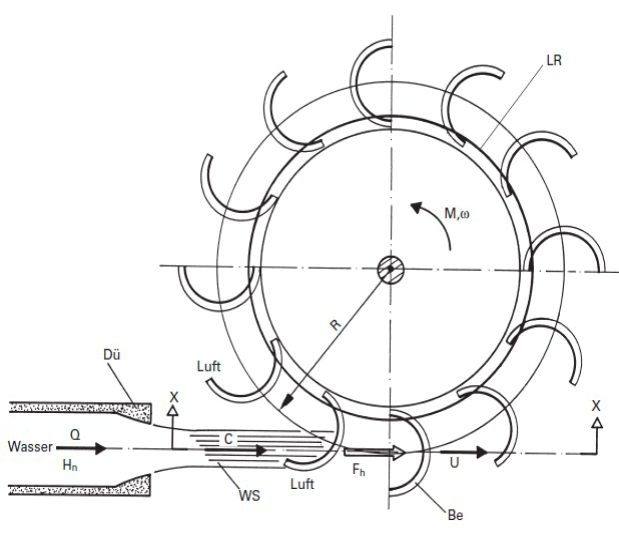
\includegraphics[width=0.98\columnwidth]{images/Pelton_Turbine_1.png}    
    \end{minipage}%
    \hfill
    \begin{minipage}[c]{0.4\columnwidth}
        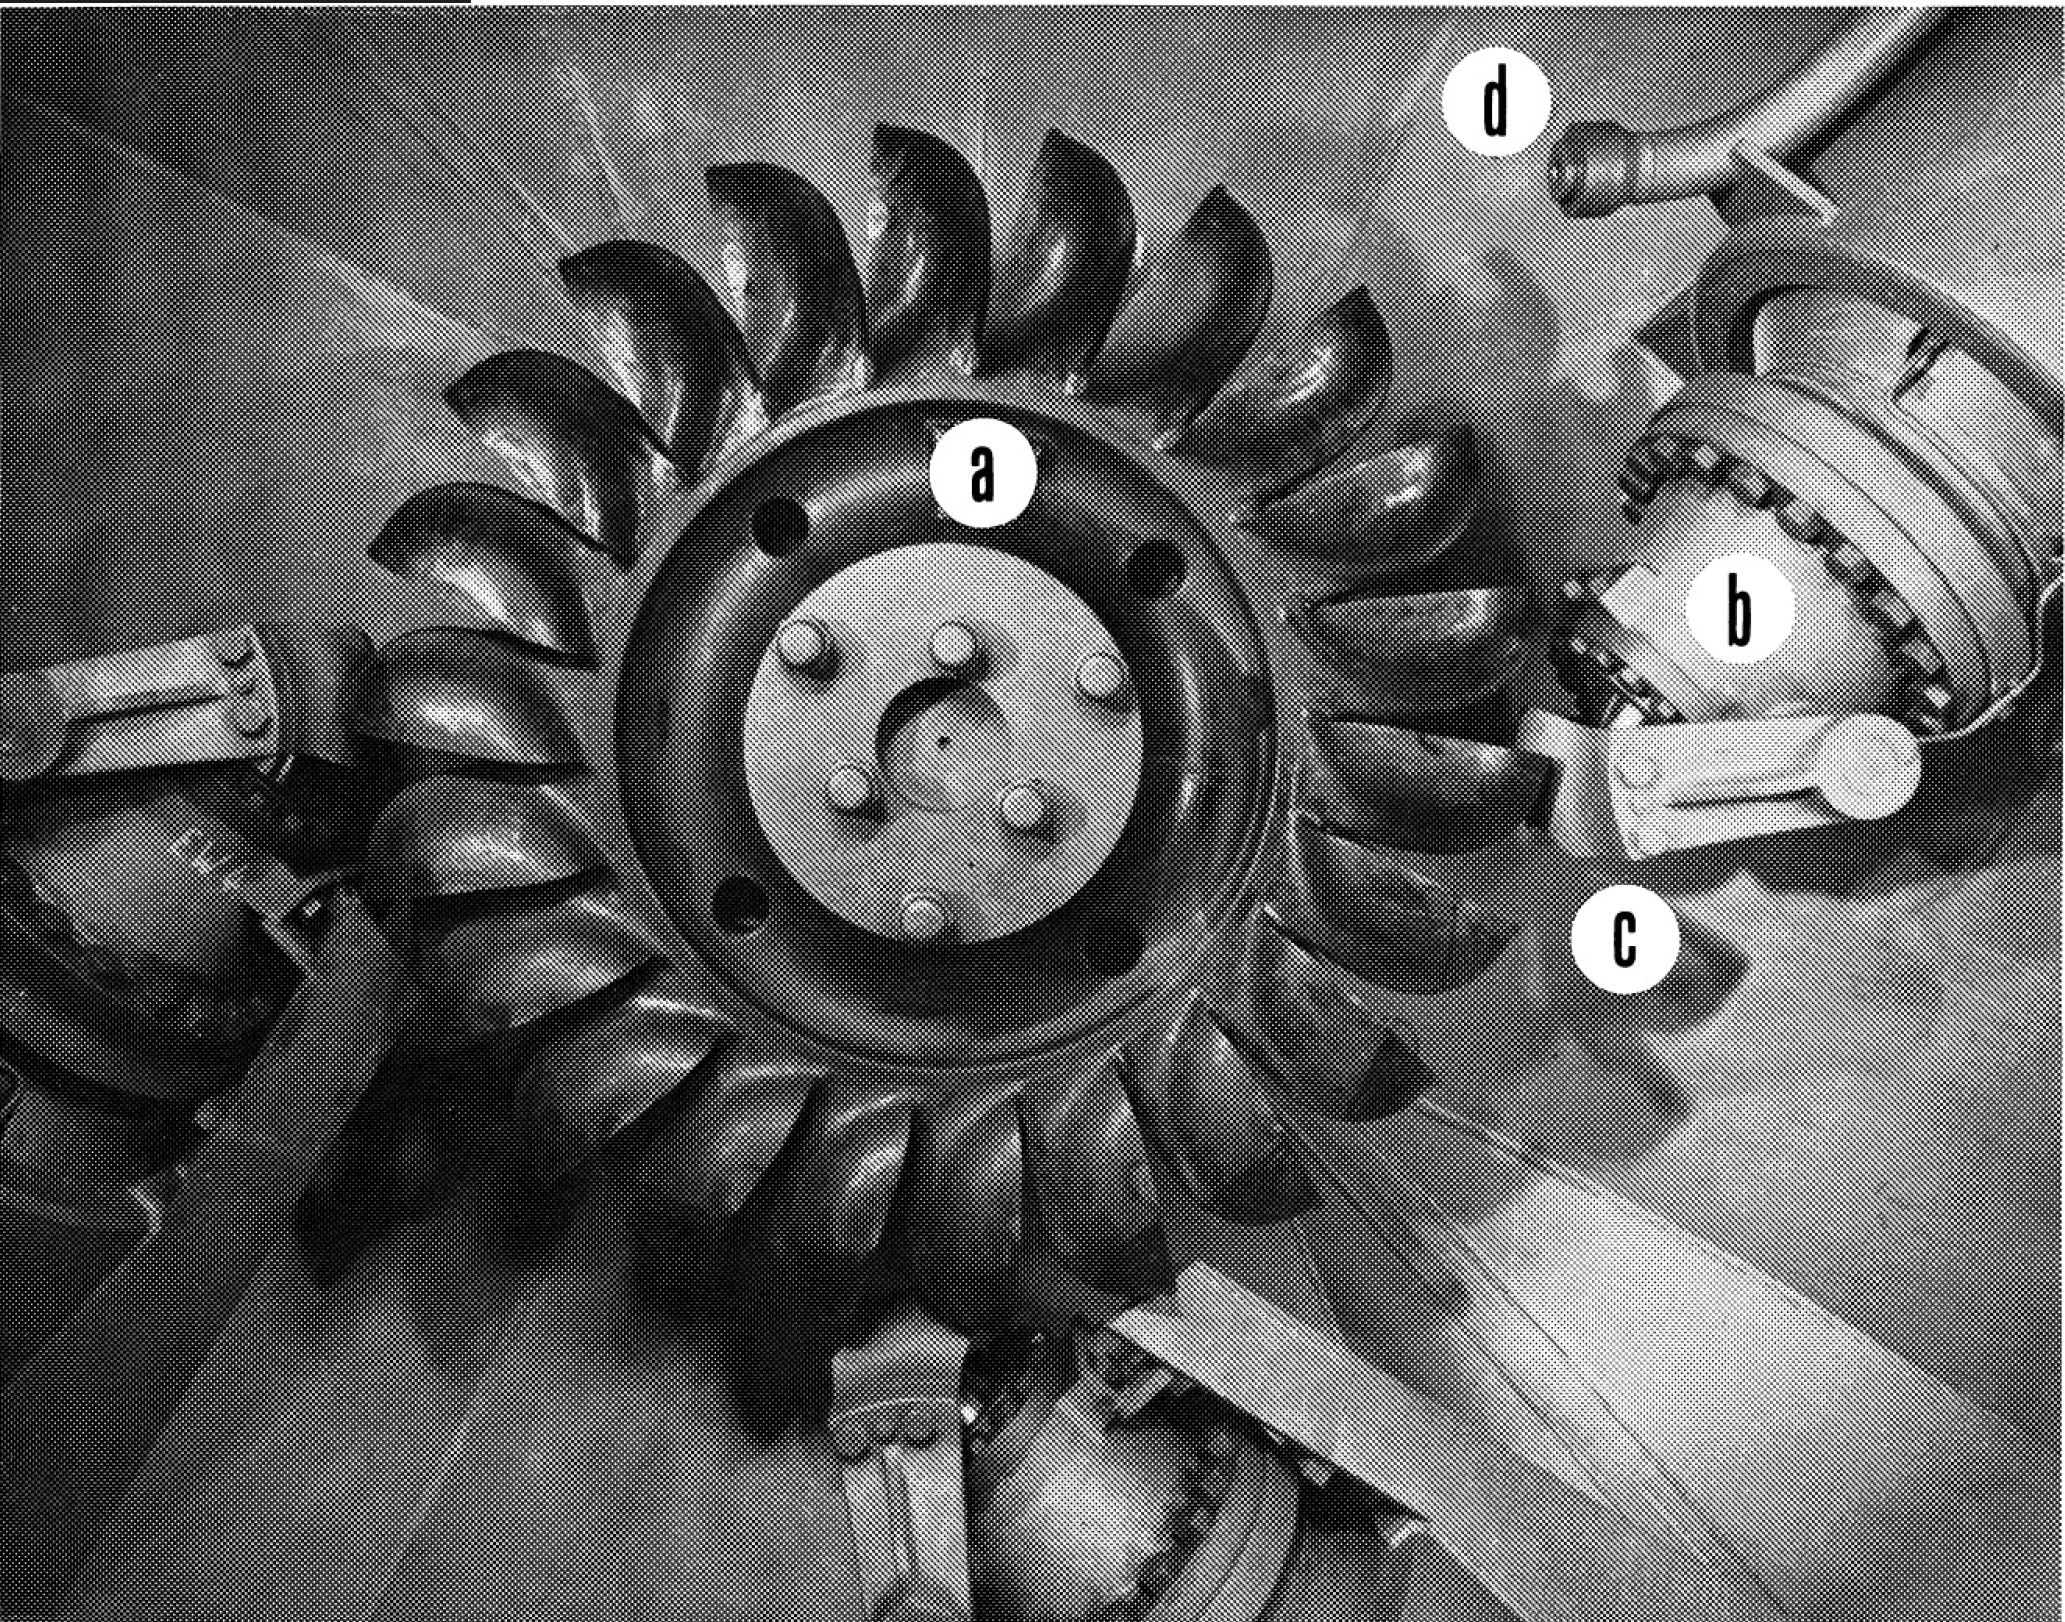
\includegraphics[width=0.98\columnwidth]{images/Pelton_Turbine_2.png}   
    \end{minipage}%
    \hfill
    \begin{minipage}[c]{0.2\columnwidth} 
        \begin{enumerate}[a)]
            \item Peltonrad
            \item Düse
            \item Strahlablenker
            \item Bremsdüse
        \end{enumerate}
    \end{minipage}

    \vspace{0.15cm}

    \begin{minipage}[c]{0.48\columnwidth}
        Düse offen    

        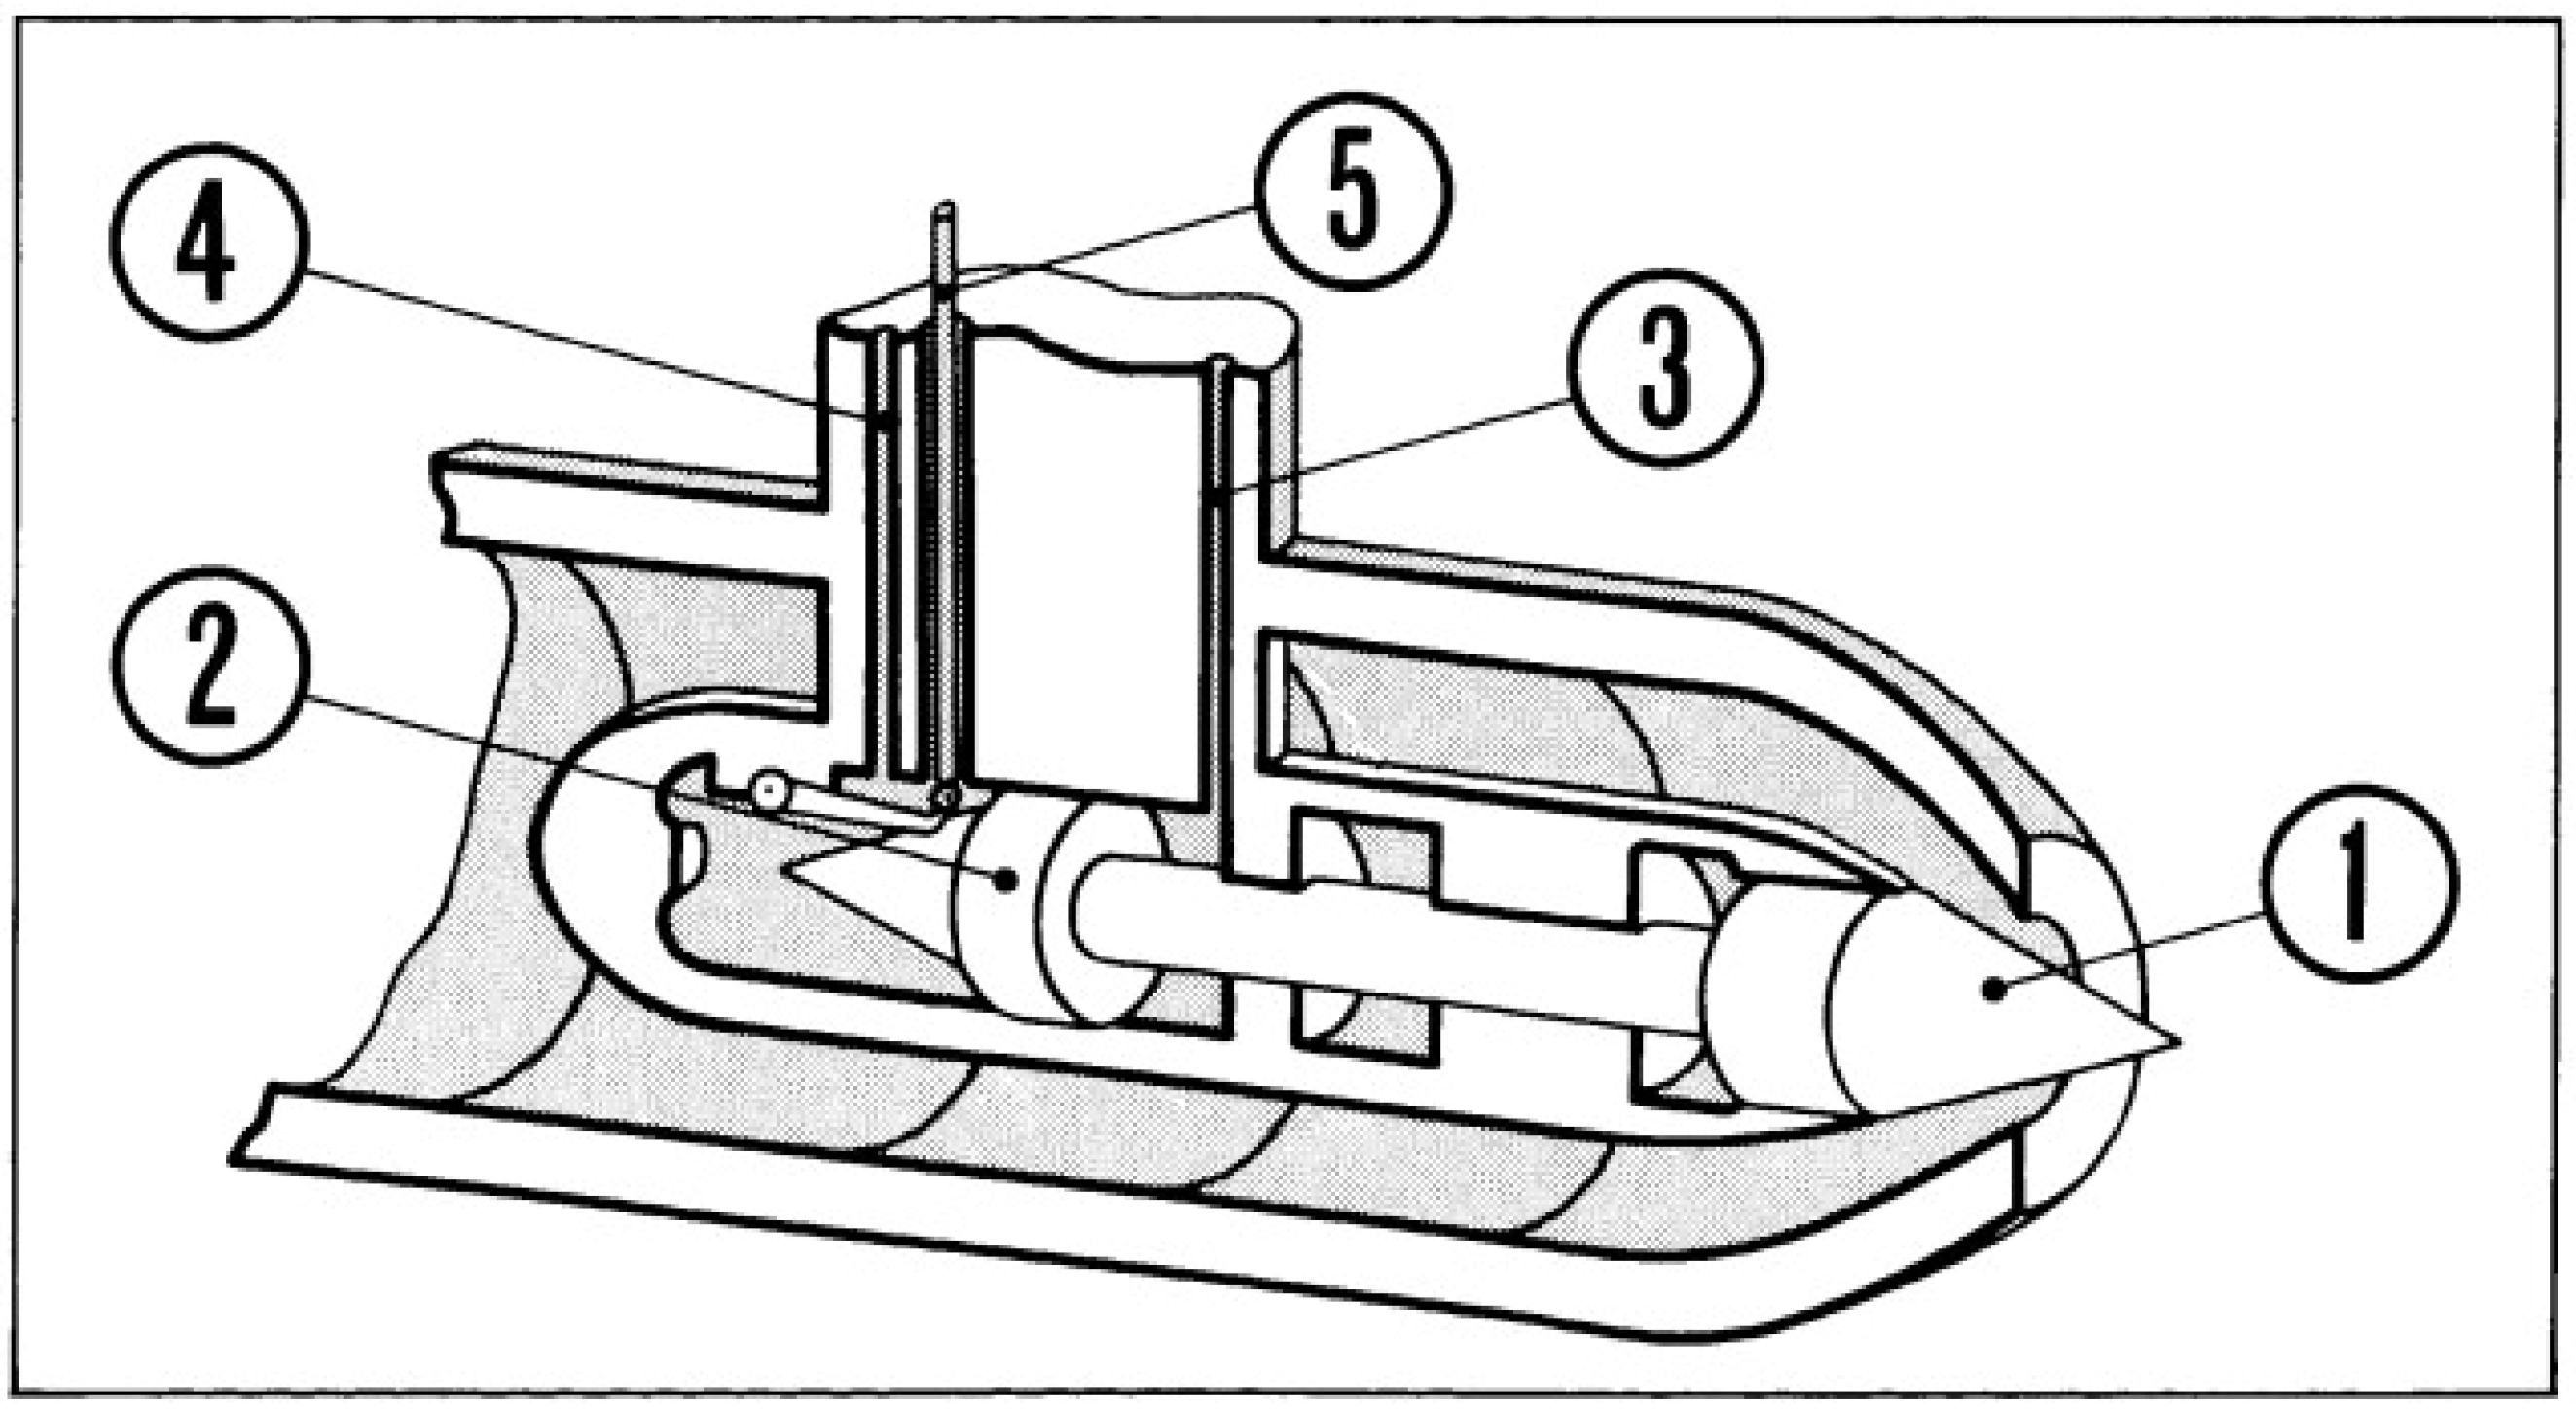
\includegraphics[width=0.98\columnwidth]{images/Pelton_Turbine_Düse_offen.png}    
    \end{minipage}
    \hfill
    \begin{minipage}[c]{0.48\columnwidth}
        Düse geschlossen   

        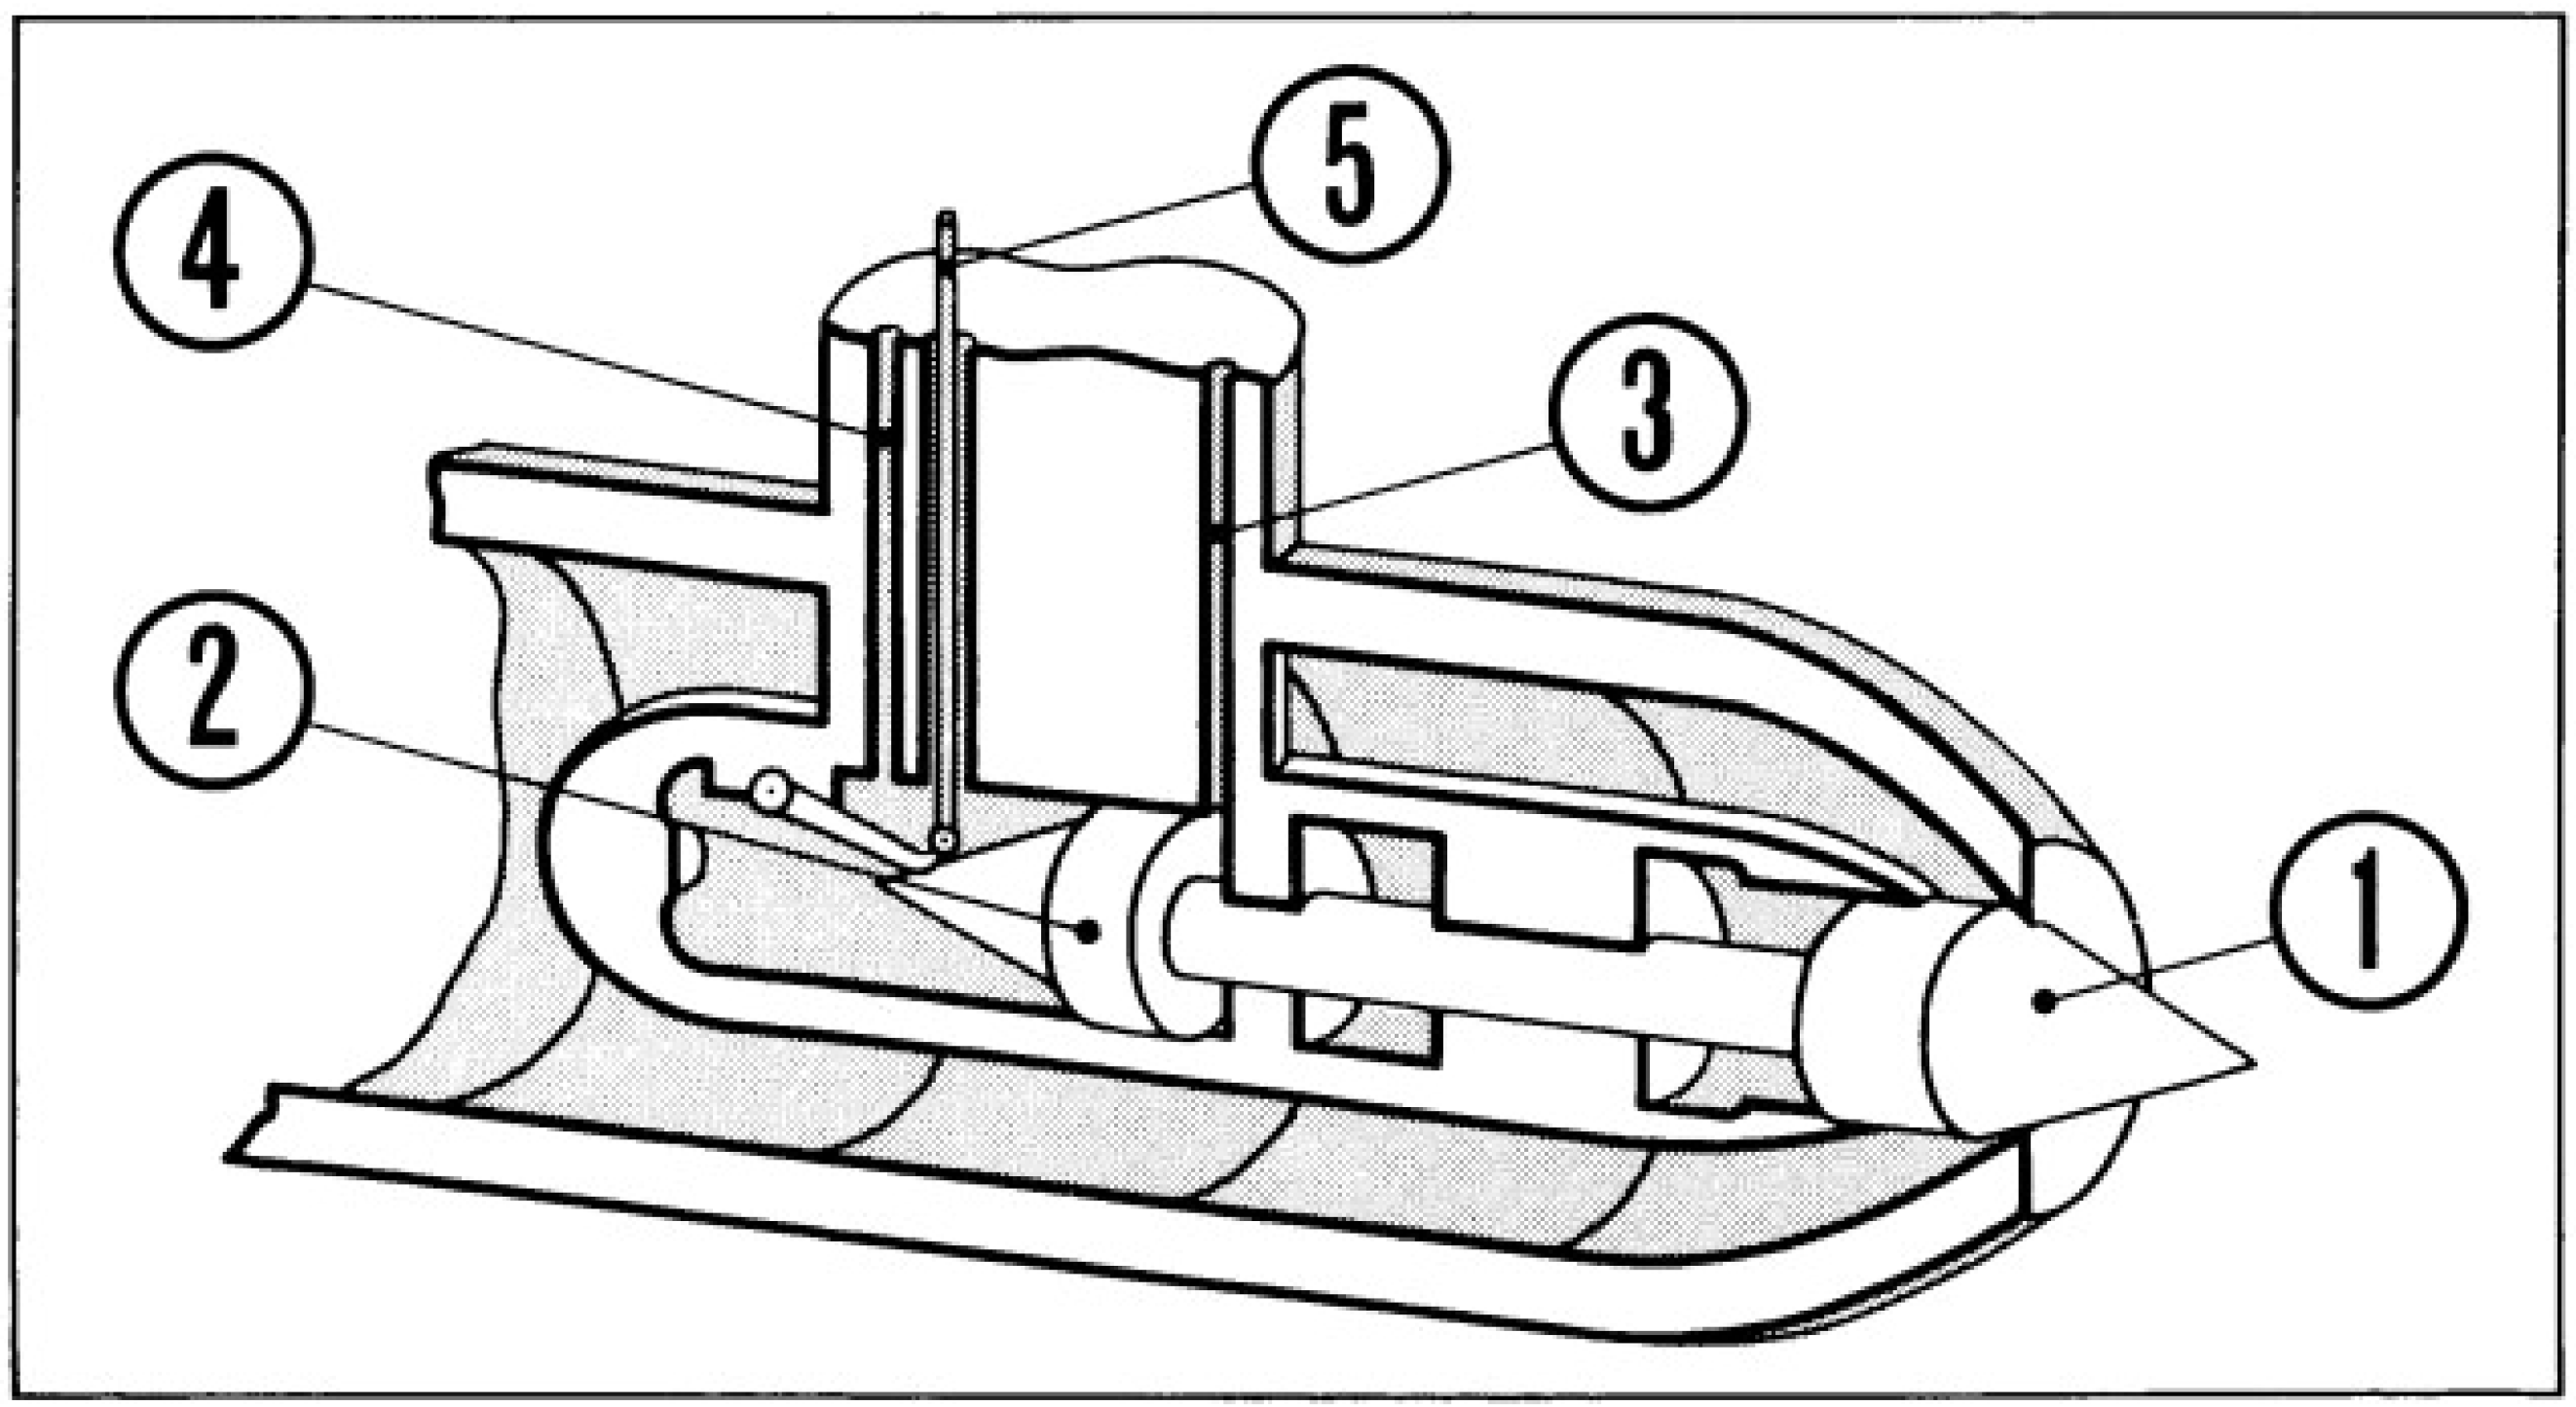
\includegraphics[width=0.98\columnwidth]{images/Pelton_Turbine_Düse_geschlossen.png}   
    \end{minipage}

    \vspace{-4mm}
    \def\columnseprulecolor{\color{white}}
    \begin{enumerate}
        \begin{multicols}{2}
            \item Düsennadel
            \item Kolben
            \item Öl zum öffnen
            \item Öl zum Schliessen
            \item Rückmeldung
        \end{multicols}
    \end{enumerate}
    \def\columnseprulecolor{\color{black}}

\subsubsection{Eingenschaften und Merkmale}
    \begin{itemize}
        \item Guter Wirkungsgrad über einen großen Einsatzbereich von 10 bis 100\% der max. Leistung
        \item Unkritische Maschine
        \item Der sogenannte Gletscherschliff muss beachtet werden (Erosion am Laufrad)
        \item Verschraubung Rad- / Generatorflansch (Kupplung) mit z.B. mechanisch vorgespannten Dehnschrauben
        \item Trockenenlegung der Kupplung
        \item Wirkungsgradverbesserungen oft möglich
        \item Rissen im Bereich der Becherwurzel (hochbelastete Zone) gilt ein spezielles Augenmerk
    \end{itemize}

    
\subsection{Reaktionsturbinen Funktionsprinzip}
    \begin{minipage}[t]{0.56\columnwidth}    
        \subsubsection{Turbinenspirale (TS)} 
            exzentrisch zur Turbinenachse angeordneter Zulaufkanal, der die durch eine \textbf{Turbinenspirale} erzeugte Drallströmung (\textbf{DS}) veranschaulicht (<<Badewannenablass>>)
        
        \subsubsection{Laufrad (LR)} 
            Schaufelrad, welches das in der \textbf{Drallströmung} DS platzierte Laufrad der Turbine darstellt
    \end{minipage}%
    \hfill
    \begin{minipage}[t]{0.43\columnwidth}
        \centering \vspace{-0.7\baselineskip}
        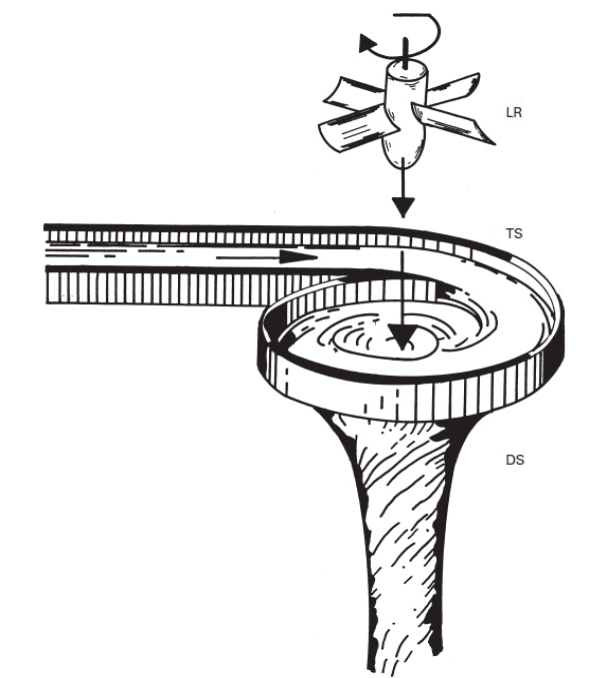
\includegraphics[width=0.9\columnwidth]{images/Laufradturbinen.png}  
    \end{minipage}
    
\subsubsection{Kavitation}
    \begin{minipage}[t]{0.65\columnwidth}
        \centering \vspace{-0.7\baselineskip}
        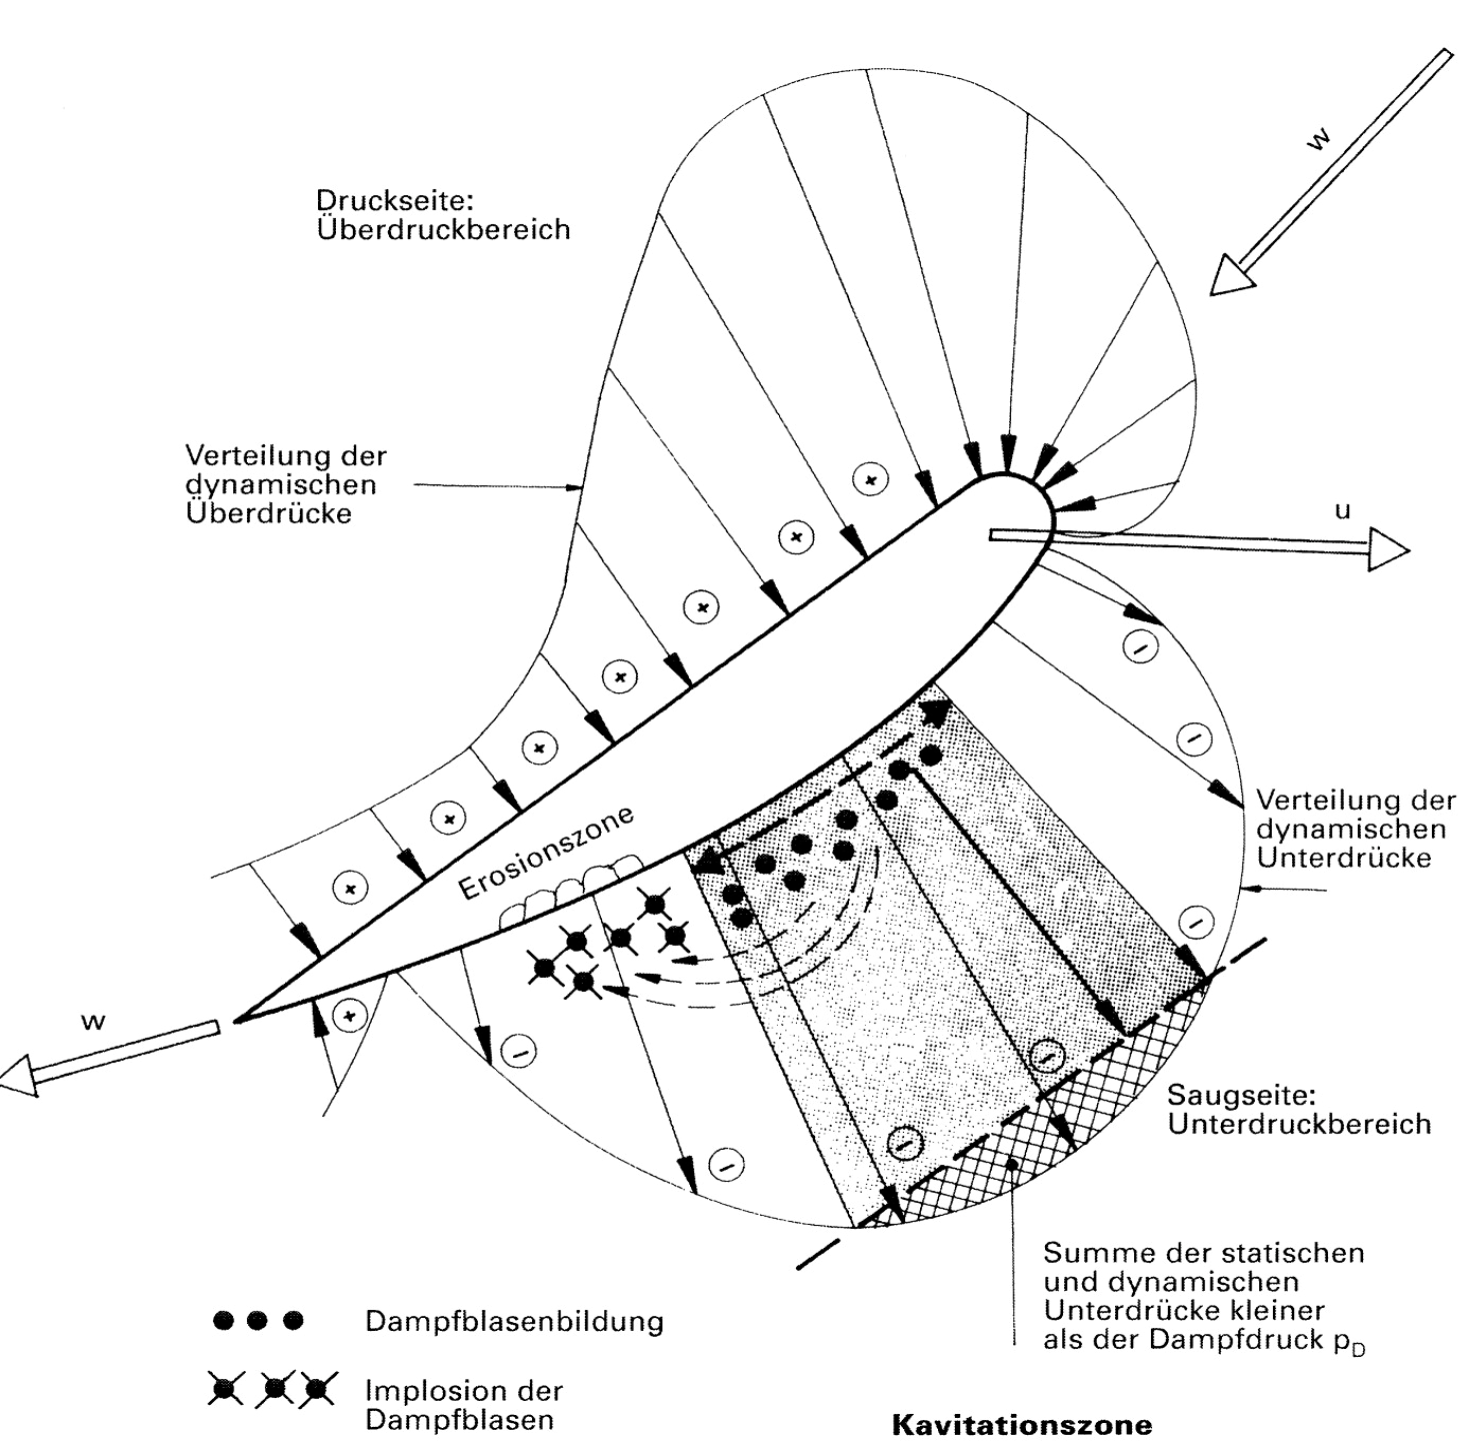
\includegraphics[width=0.95\linewidth]{images/Kavitation.png}
    \end{minipage}%
    \hfill
    \begin{minipage}[t]{0.34\columnwidth}
        \begin{itemize}
            \item[$w$] Rel. Geschw. des Wassers 
            \item[$u$] Umfanggeschw. der Schaufel
        \end{itemize}
    \end{minipage}  
    
    \vspace{0.15cm}
    
    \begin{tabular}{ll}
        \toprule[.13em]
        \textbf{Turbinentyp} & \({n_D}/{n_N}\) \\
        \midrule
        Francis, \(n_q = 40 \ldots 80\) U/min                       & \(1.7 \ldots 2.0\) \\
        Francis, \(n_q = 80 \ldots 120\) U/min                      & \(2.0 \ldots 2.2\) \\
        Propeller, feste Lauf- und Leitschaufeln                    & \(1.8 \ldots 2.2\) \\
        Kaplan, verstellbare Laufschaufeln, feste Leitschaufeln     & \(2.4 \ldots 2.8\) \\
        Kaplan, verstellbare Lauf- und Leitschaufeln                & \(2.4 \ldots 3.2\) \\
        Pumpen im Turbinenbetrieb, \(n_q = 30 \ldots 100\) U/min    & \(1.4 \ldots 1.8\) \\
        \bottomrule[.13em]
    \end{tabular}
    
    \vspace{0.15cm}
    
    Je grösser \({n_D}/{n_N}\), desto stärker muss die Turbine dimensioniert werden
    
    \newcolumn
    
    \textbf{Verhältnis der Volumenströme bei Durchgangs- bzw. Nenndrehzahl:}

    \begin{minipage}[t]{0.49\columnwidth}
        $\begin{aligned}
            n_q < 100 \ \mathrm{U/min:} & \quad Q_D < Q_N \\
            n_q = 100 \ \mathrm{U/min:} & \quad Q_D = Q_N \\
            n_q > 100 \ \mathrm{U/min:} & \quad Q_D > Q_N 
        \end{aligned}$
    \end{minipage}%
    \hfill
    \begin{minipage}[t]{0.49\columnwidth}
        \begin{itemize}
            \item \textbf{Durchgangsdrehzahl} \(n_D\)
            \item \textbf{Nenndrehzahl} \(n_N\)
            \item \textbf{Spezifische Drehzahl} \(n_q\)
        \end{itemize}
    \end{minipage}

    \renewcommand{\arraystretch}{1.2} % Erhöht Zeilenhöhe für bessere Lesbarkeit
    \begin{tabular}{@{} l p {7cm} l @{}}
        $[n_D]$   & Drehzahl bei Lastabwurf (plötzlicher Generatorverlust)  \dotfill & $\mathrm{\frac{U}{min}}$ \\
        $[n_N]$   & Tatsächliche Drehzahl im Normalbetrieb                    \dotfill & $\mathrm{\frac{U}{min}}$ \\
        $[n_q]$   & Drehzahl einer skalierten Maschine  \(\left(H = 1\,\mathrm{m},\, Q = 1\,\mathrm{m}^3/\mathrm{s}\right)\) \dotfill & $\mathrm{\frac{U}{min}}$ \\
    \end{tabular}
    
\subsection{Francisturbinen}
    \begin{minipage}[t]{0.48\columnwidth}
        \centering \vspace{-0.7\baselineskip}
        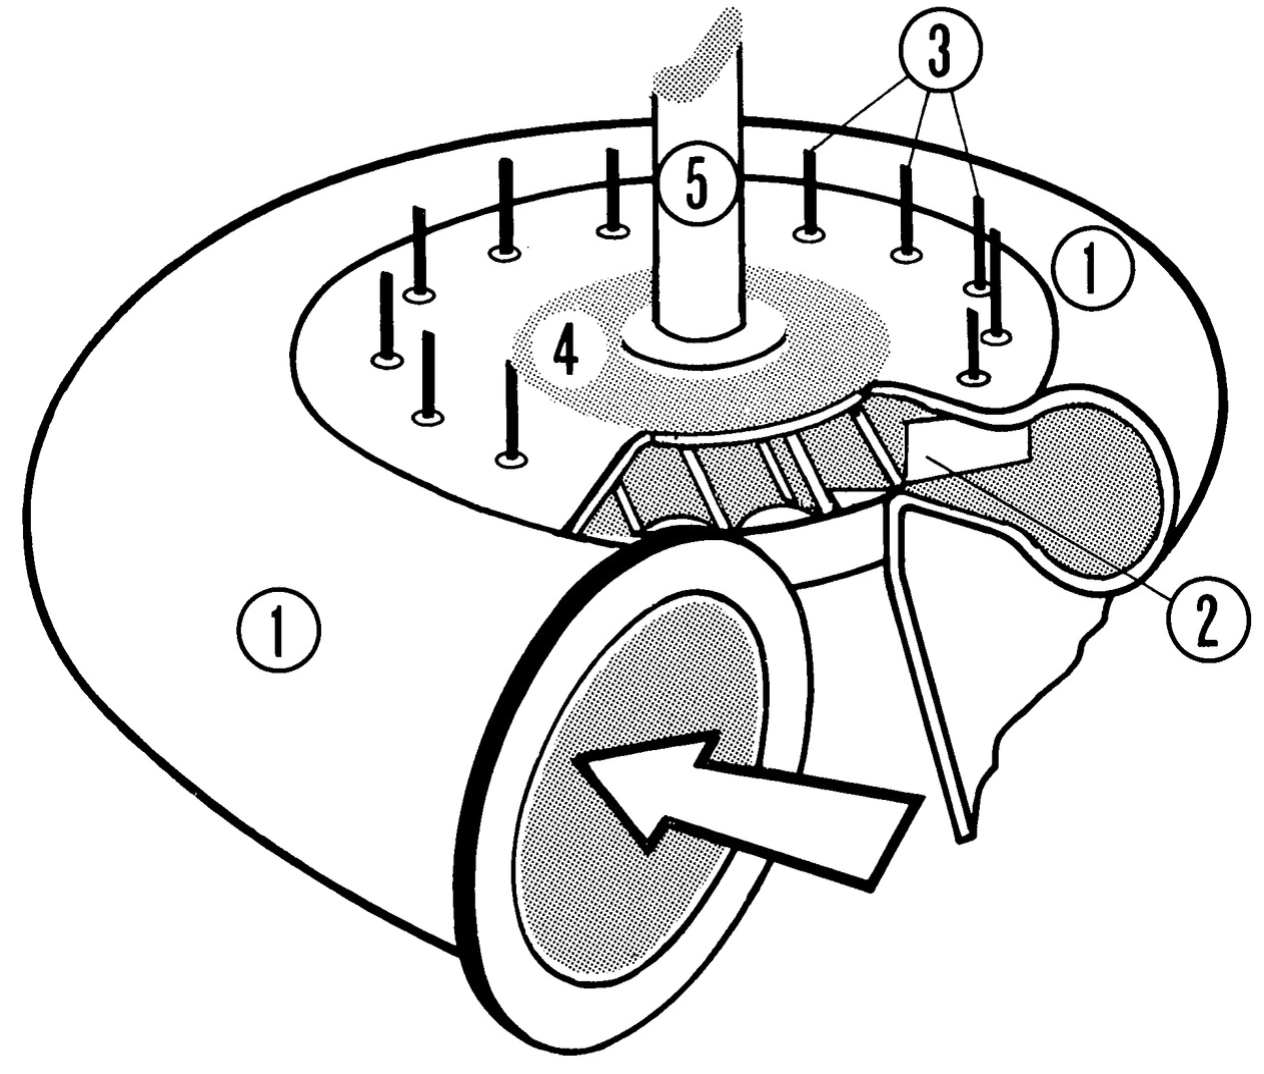
\includegraphics[width=0.85\columnwidth]{images/Francis_Turbine.png}    
    \end{minipage}
    \hfill
    \begin{minipage}[t]{0.48\columnwidth}
        \begin{enumerate}
            \item Einlaufspirale
            \item Leitschaufeln
            \item Leitschaufelnachse
            \item Laufrad
            \item Turbinenwelle
        \end{enumerate}  
    \end{minipage}

\subsection{Kaplanturbinen}
    \begin{minipage}[t]{0.48\columnwidth}
        \centering \vspace{-0.7\baselineskip}
        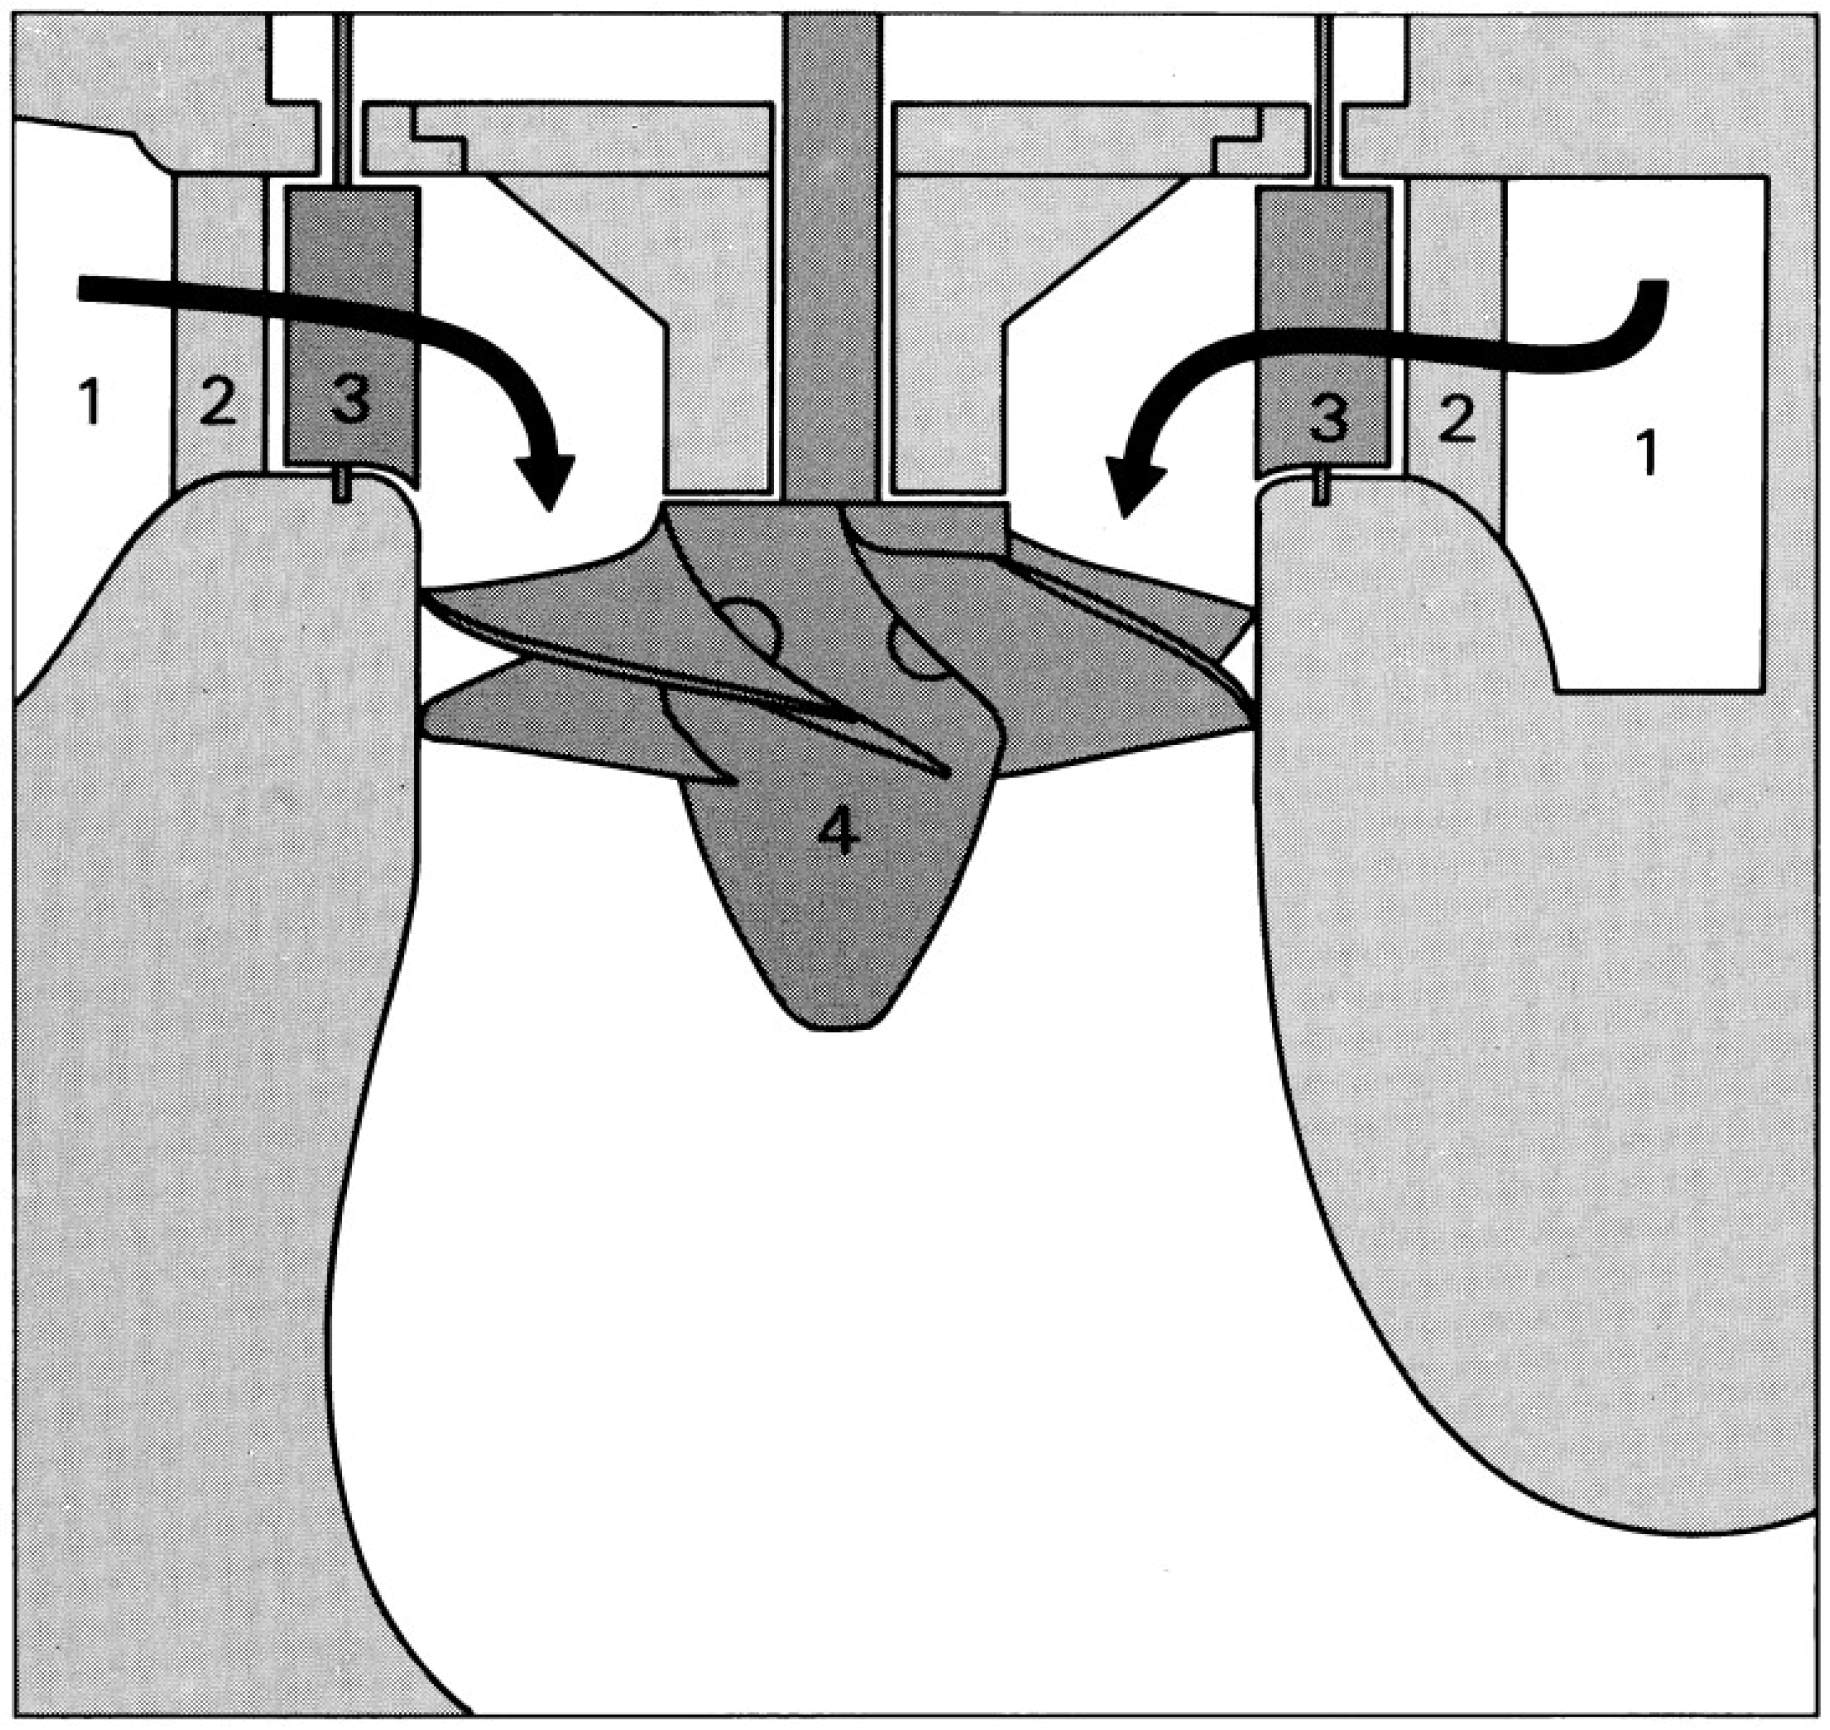
\includegraphics[width=0.85\columnwidth]{images/Kaplan_Turbine.png}    
    \end{minipage}
    \hfill
    \begin{minipage}[t]{0.48\columnwidth}
        \begin{enumerate}
            \item Einlaufspirale
            \item Stützschaufeln
            \item Leitschaufeln
            \item Kaplan-Rad
        \end{enumerate}  
    \end{minipage}

\subsection{Rohrturbinen (horizontale Kaplanturbinen)}
    \begin{minipage}[t]{0.48\columnwidth}
        \centering \vspace{-0.7\baselineskip}
        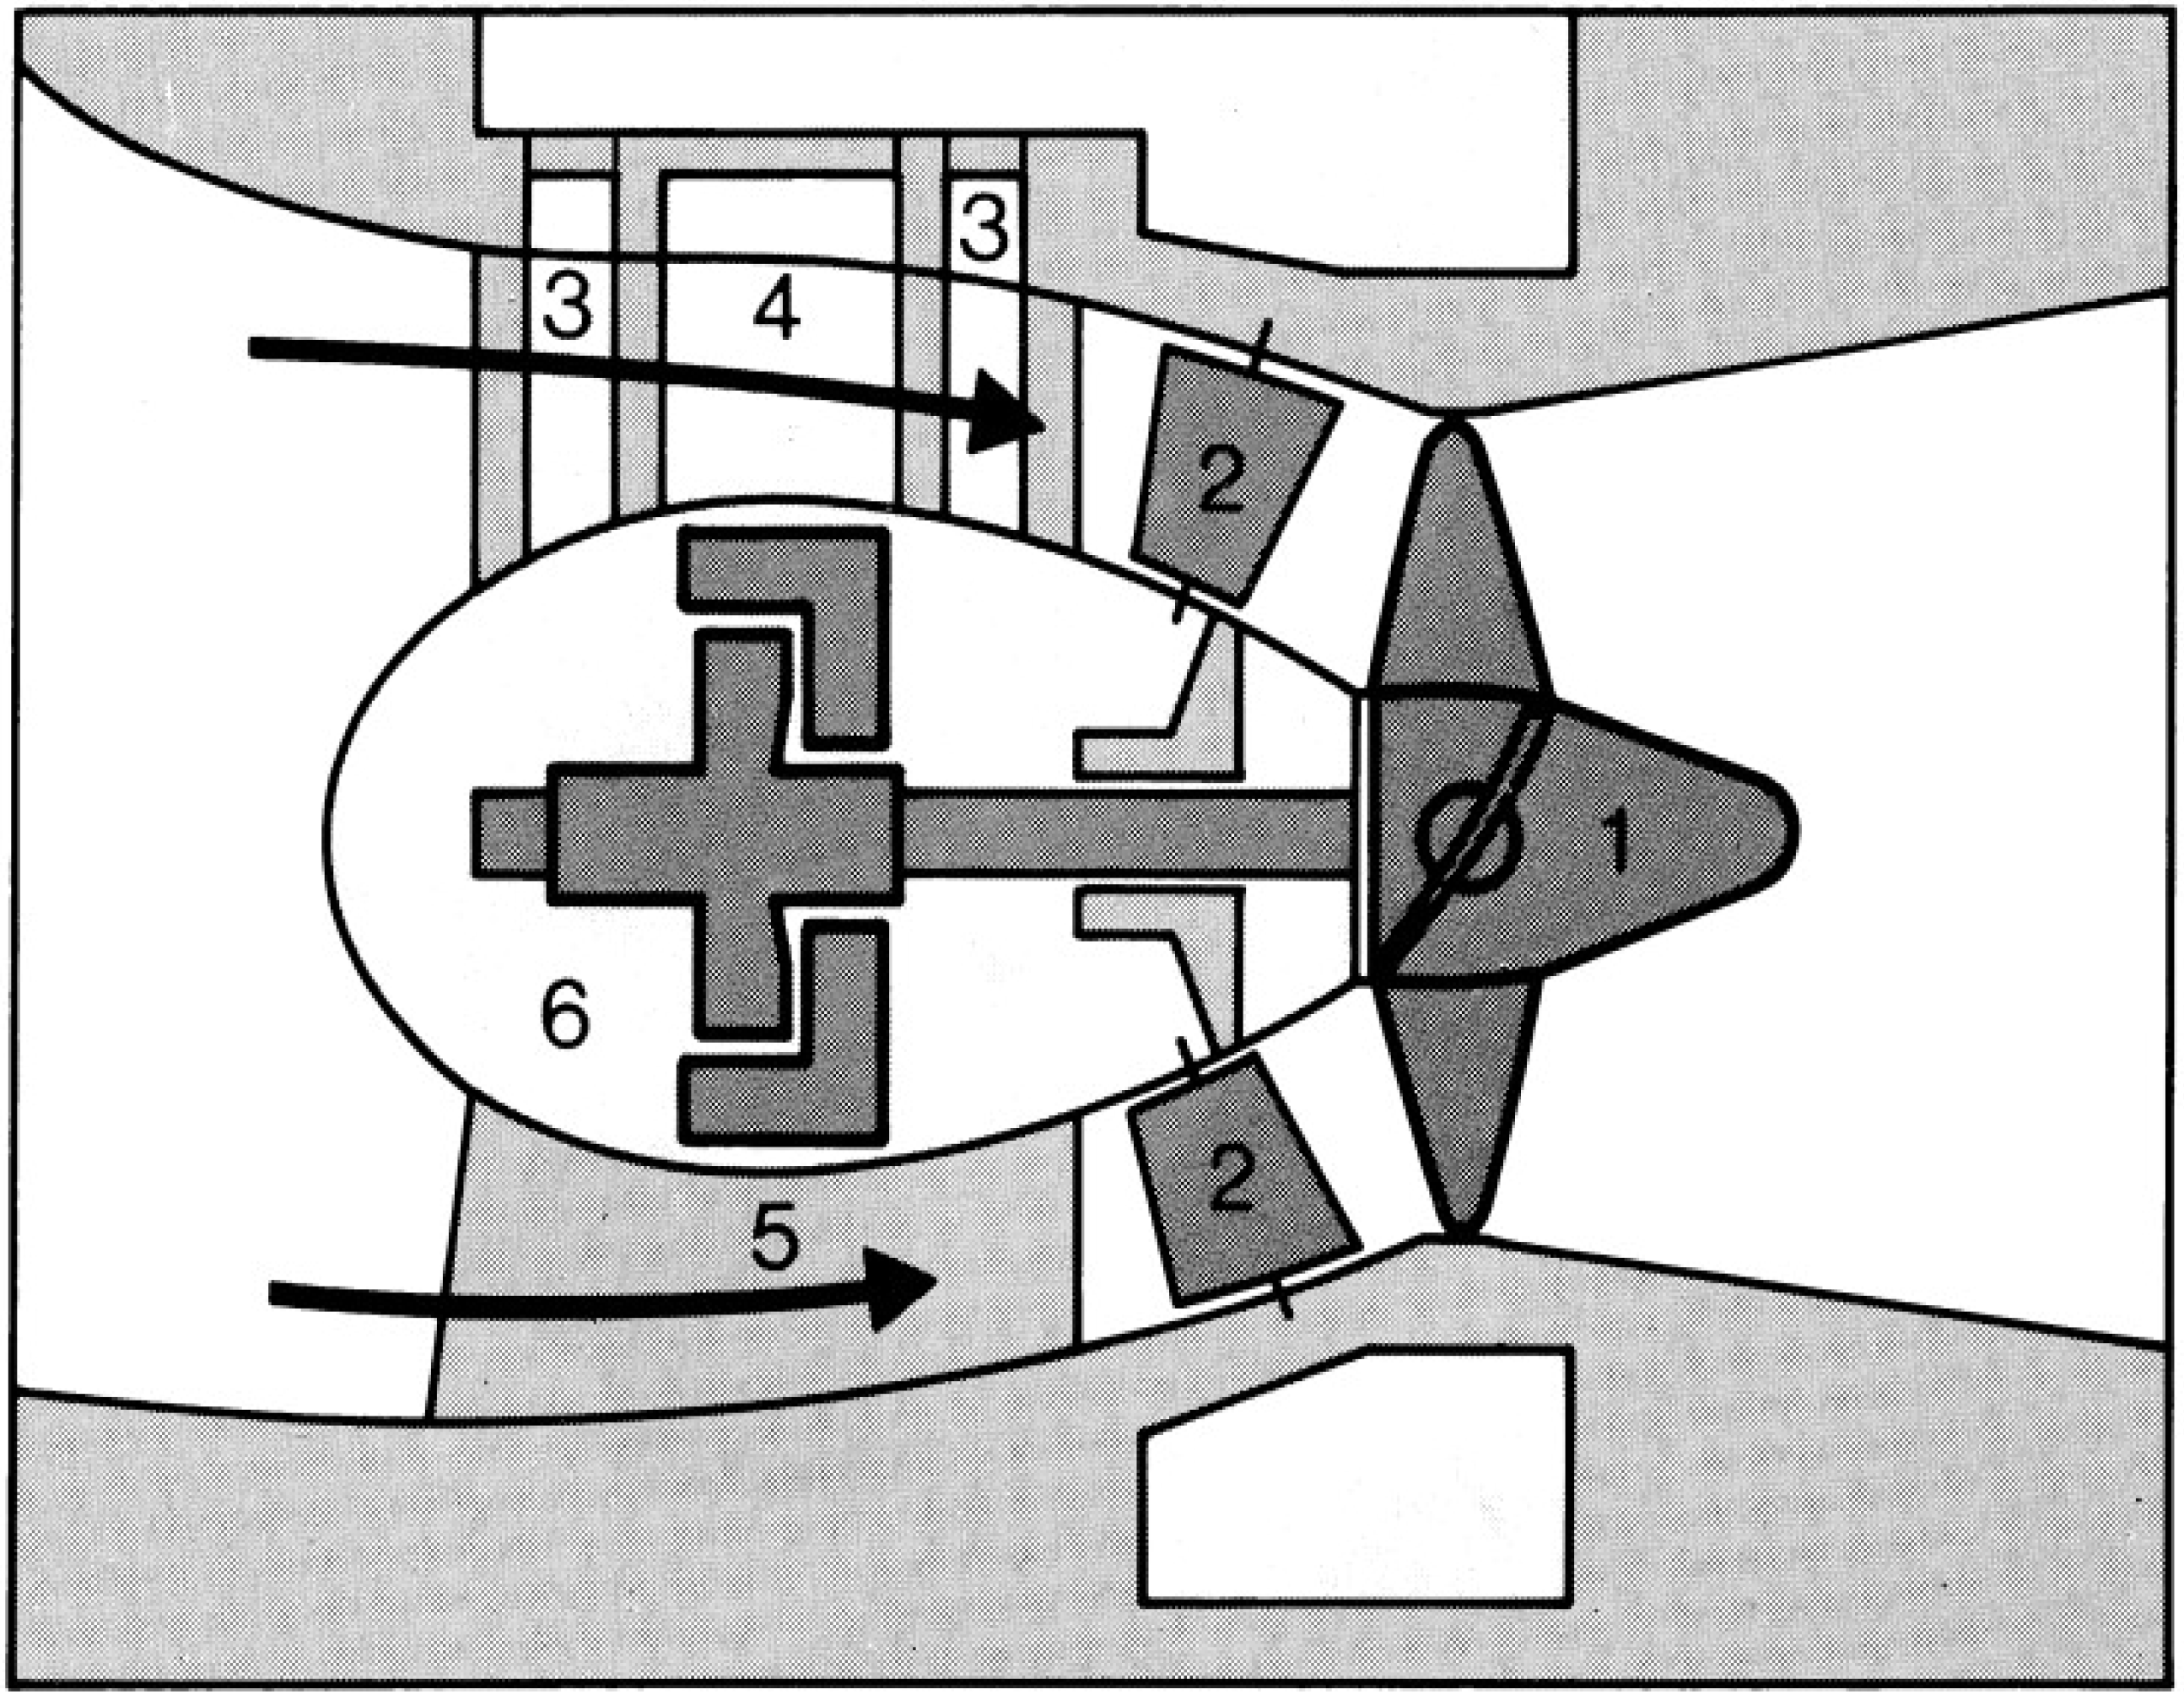
\includegraphics[width=0.85\columnwidth]{images/Rohr_Turbinen.png}    
    \end{minipage}
    \hfill
    \begin{minipage}[t]{0.48\columnwidth}
        \begin{enumerate}
            \item Schaufelrad
            \item Leitschaufeln
            \item Zustiegsschächte
            \item Demontageschacht
            \item Sockel
            \item Generator
        \end{enumerate}  
    \end{minipage}

\subsection{Strafloturbinen}
    \begin{minipage}[t]{0.48\columnwidth}
        \centering \vspace{-0.7\baselineskip}
        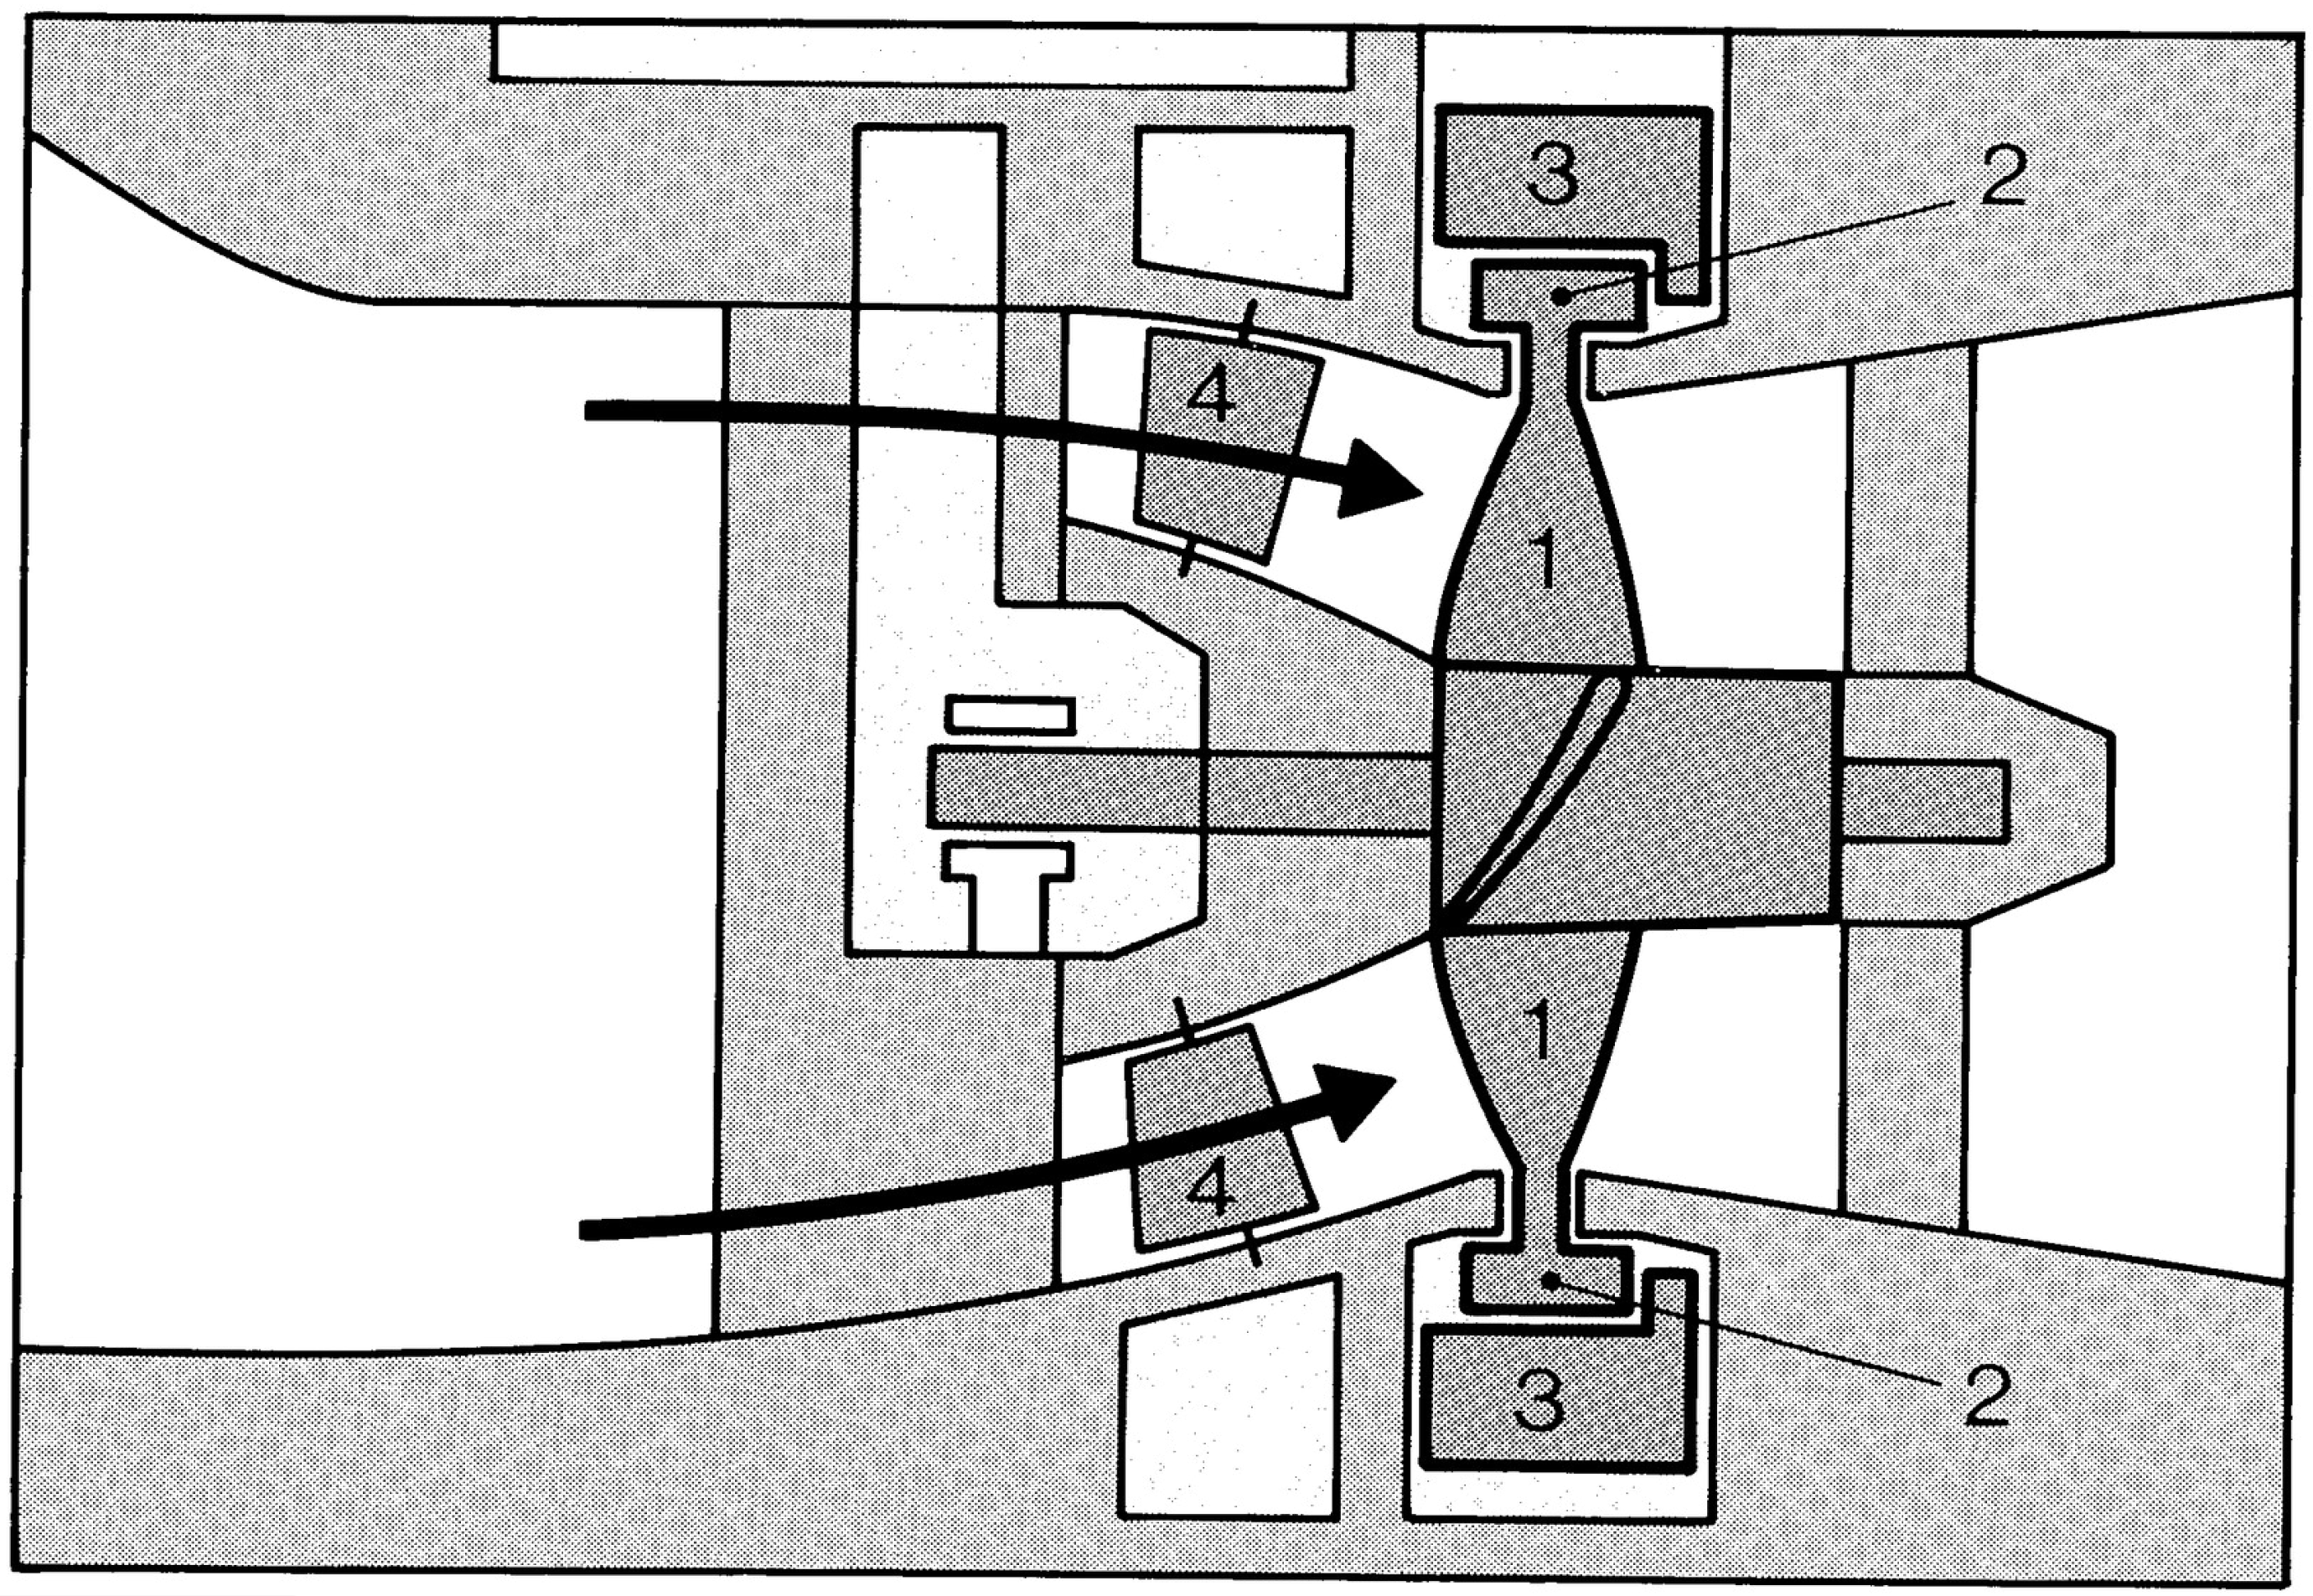
\includegraphics[width=0.85\columnwidth]{images/Straflo_Turbine.png}    
    \end{minipage}
    \hfill
    \begin{minipage}[t]{0.48\columnwidth}
        \begin{enumerate}
            \item Laufradschaufeln
            \item Rotor, Pole des Generators
            \item Stator
            \item Leitschaufeln
        \end{enumerate}  
    \end{minipage}

\subsection{Speicherpumpen und Pumpturbinen}
    \begin{center}
        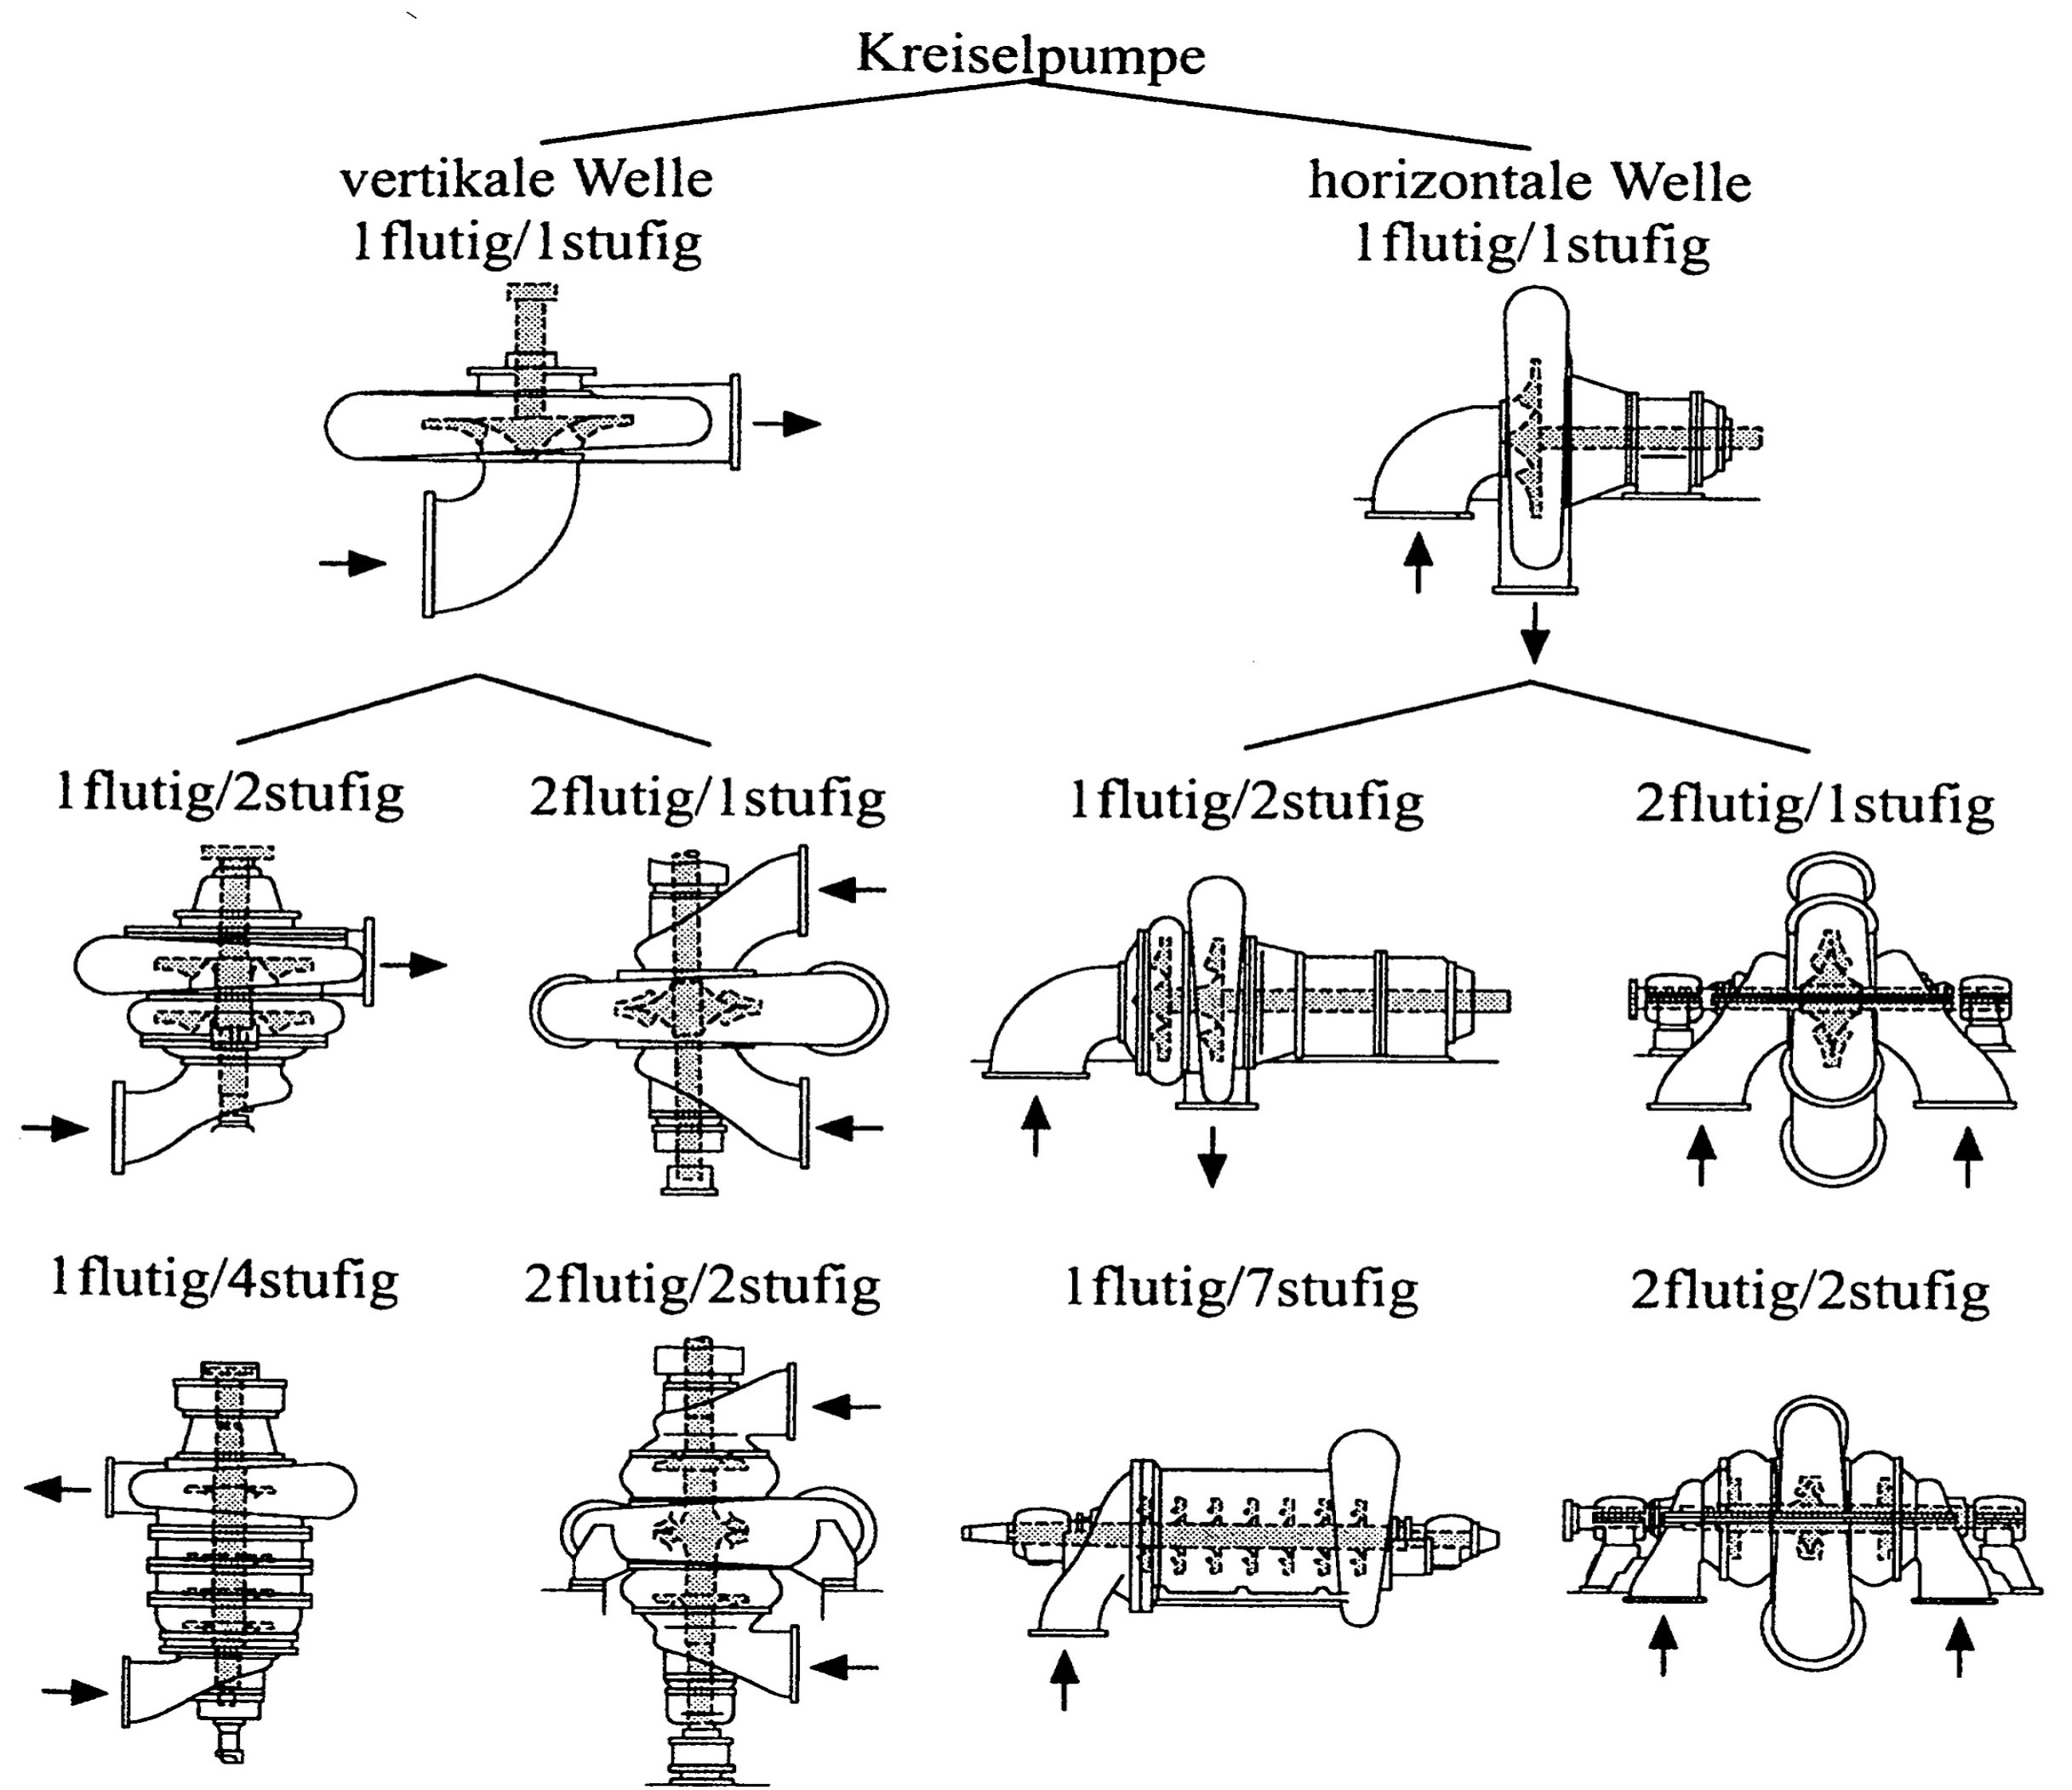
\includegraphics[width=0.9\columnwidth]{images/Speicherpumpen und Pumpturbinen.png}   
    \end{center}

\subsubsection{Dreimaschinensatz}
    Besteht aus: Generator/Motor, Francisturbine und Speicherpumpe

    \vspace{0.1cm}

    \textcolor{red}{\textbf{Nachteile}} 
    \begin{itemize}
        \item Zwei hydraulische Maschinen sowie eine größere Anzahl Abschlussorgane sind nötig.
    \end{itemize}
    \textcolor{green}{\textbf{Vorteil}}
    \begin{itemize}
        \item Unabhängige Optimierung der Turbine und der Pumpe ist möglich.
    \end{itemize}

\subsection{Wahl des Generators}
    Der Generator muss synchron mit dem Netz drehen. Daher muss die definitive Drehzahl der in der Nähe liegenden Synchrondrehzahl entsprechen.

    \vspace{0.15cm}

    \begin{minipage}[t]{0.35\columnwidth}\vspace*{-2mm}
        $\boxed{n = 60 \cdot \frac{f}{p} = \frac{3000}{p}}$
    \end{minipage}%
    \hfill
    \begin{minipage}[t]{0.64\columnwidth}\vspace*{-2mm}
        \renewcommand{\arraystretch}{1.2}
        \begin{tabular}{@{} l p {3.6cm} l @{}}
            $[n]$ & Drehzahl des Generators \dotfill  & $\text{U/min}$ \\
            $[f]$ & Frequenz, meist 50 Hz \dotfill    & $\text{Hz} = \frac{1}{\text{s}}$ \\
            $[p]$ & Polpaarzahl \dotfill              & (1, 2, 3, \dots) \\
        \end{tabular}
    \end{minipage}

\subsection{Kochrezept zur Grob-Auslegung von Pumpen und Turbinen}

\begin{enumerate}
    \item Bestimmung der \textbf{Netto-Fallhöhe} \( H_n \)
    \item Auswahl \textbf{Gesamtdurchfluss} \( Q \), abhängig von Zufluss, Rückhaltemöglichkeit, Einsatztyp (z.B. Spitzenlast)
    \item Bestimmung der \textbf{hydraulischen Leistung} mithilfe der \textbf{elektrischen Leistung} $P_{el} $ und dem Gesamtwirkungsgrad $\eta_{tot}$ :
    \[
    P_\mathrm{hyd} = \rho \cdot Q \cdot g \cdot H_n = \frac{P_{el}}{\eta_{tot}}
    \]
    \item Auswahl \textbf{Turbinentyp}, \textbf{Turbinen-Durchfluss} \( Q \) und \textbf{spezifische Drehzahl} \( n_q \) aus Diagrammen\\
    (ggf. Aufteilung \( Q \) auf mehrere Turbinen / Pumpen)
    \item Bestimmung der \textbf{Turbinen-Drehzahl}:
    \[
    n = n_q \cdot \frac{H_n^{3/4}}{Q^{1/2}}
    \]
    \item Bestimmung der \textbf{Polpaarzahl}:
    \[
    p = \frac{3000}{n}
    \]
    (auf ganze Zahl runden und prüfen, ob \( n_q \) nach Rundung noch im möglichen Bereich liegt)
    \item Weitere Bedingungen zur \textbf{Feinauslegung}:
    \begin{itemize}
        \item Teillastverhalten, Wirkungsgrad, Betriebsbereiche
        \item Räumliche Bedingungen, Simulationen, Experimente
        \item \(\ldots\)
        \item Lösung ist ein Abwägen und iterativer Prozess
    \end{itemize}
\end{enumerate}
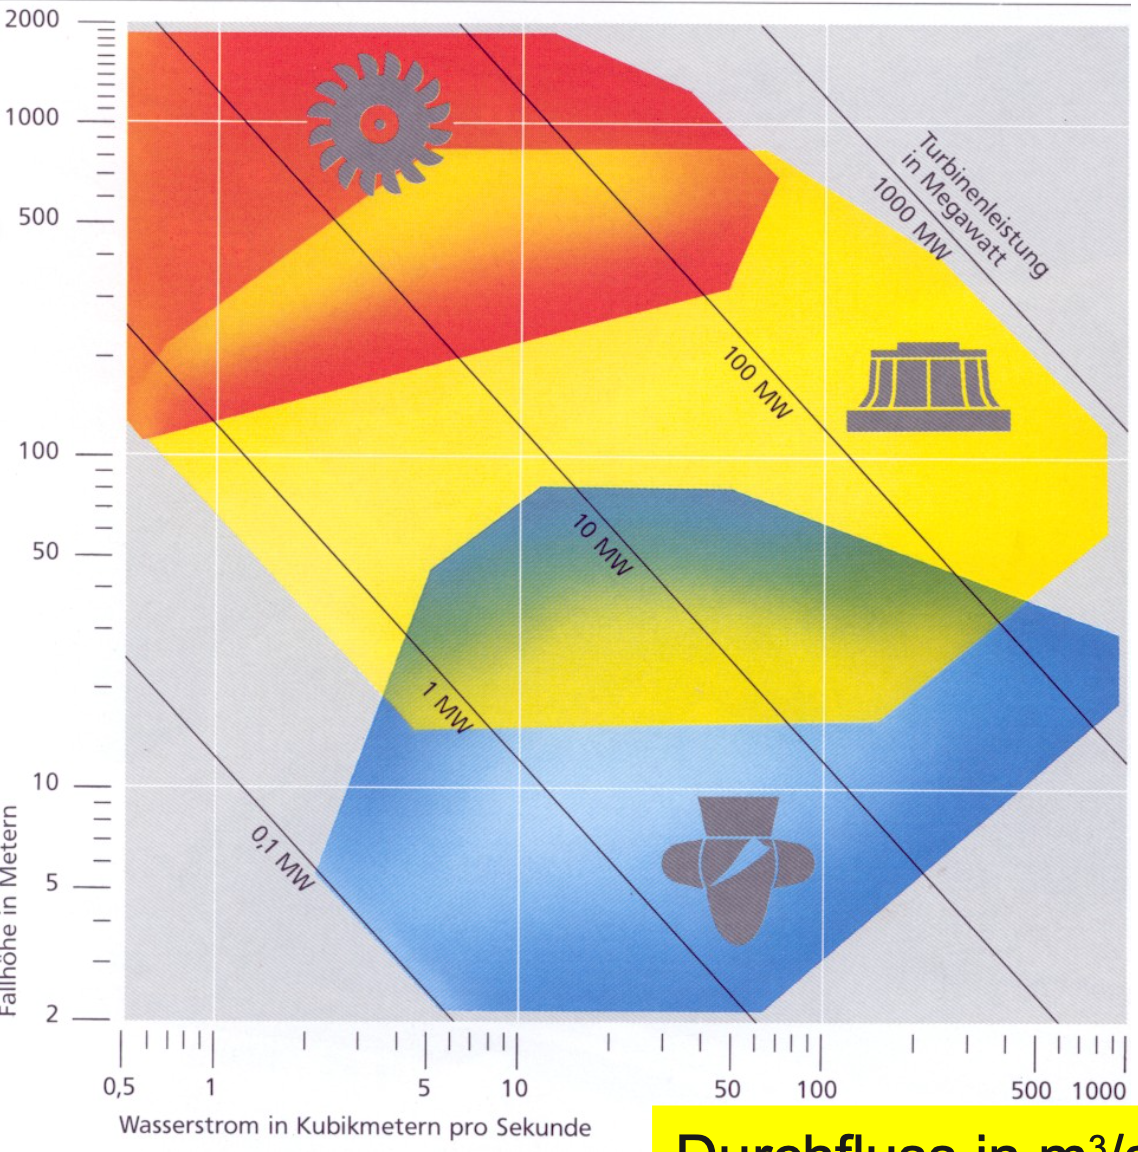
\includegraphics[width=1\linewidth]{images/Turbinentypen.png}
\textcolor{red}{Peltonturbine}, \textcolor{yellow}{Francisturbine}, \textcolor{blue}{Kaplanturbine}

\newcolumn
